\documentclass[12pt,oneside]{book}

\newcommand\coursename{BookML in University of Edinburgh}
\newcommand\coursecode{MATXXXXXXX}
\newcommand\courseauthor{Steven O'Hagan, Hayden Maudsley-Barton, and Charlotte Desvages}
\newcommand\courseyear{2024--25}
\newcommand\coursedescription{A description of the course.}

%%% School of Mathematics preamble for HTML course notes with BookML.
%%% Adapted directly from https://github.com/vlmantova/bookml/tree/main/template

%%% This template imports all the most commonly requested packages which have been
%%% tested and are compatible with BookML. You can comment out any \usepackage
%%% commands that you are not using in your document.

%%% You should import extra packages, define custom macros and environments,
%%% etc in preamble/custom.tex.


%% BookML and template settings

%%% RECOMMENDED
% better accented letters and ligatures in PDF
\usepackage[T1]{fontenc}
% set language of outputs
\usepackage[british]{babel}
% PDF hyperlinks and metadata
\usepackage[pdfusetitle]{hyperref}
% higher quality variant of Computer Modern
%\usepackage{lmodern}

%%% REQUIRED for correct formatting and tagging of BookML output: title and author
\title{\coursename}
\author{\courseauthor}
\date{\courseyear}

%%% OPTIONAL but highly recommended
% additional BookML and LaTeXML functionality
\usepackage{bookml/bookml}
% additional versions of the document (e.g. large print) for inclusion in the HTML output
\bmlAltFormat{\jobname.pdf}{PDF (sans serif)} % this version is always included unless it's given an empty name
\bmlAltFormat{\jobname-serif.pdf}{PDF (serif)}
% simple way of generating a large print PDF (~19% bigger) without changing pagination


% short text description used for PDF and SCORM metadata
\hypersetup{pdfsubject={\coursedescription}}

% Provide \alttext (easier to remember)
\providecommand\alttext{\bmlDescription}

%%% REQUIRED for TikZ: use bmlImageEnvironment for TikZ and other images, since
%%%                    LaTeXML is slow and often produces garbled TikZ output
%%%                    (this requires \usepackage{bookml/bookml})
% tell BookML to compile tikzpicture and tikzcd environments into images via LaTeX
\bmlImageEnvironment{tikzpicture}


\iflatexml          % are we compiling HTML through LaTeXML?
    
\else               % are we compiling the PDF?
    
\fi

\usepackage{pgfplots}  % this also loads TikZ
\usepackage[all]{xy}

%% Packages

% Font-related
\usepackage{amsmath,amsfonts,amssymb,amsthm}
\usepackage{bm}
\usepackage[normalem]{ulem}

% Bibliography: note that only natbib is compatible at present
\usepackage[square,sort,comma,numbers]{natbib} %\usepackage{natbib}

% Images (note that TikZ and vector graphics/diagrams packages
% are imported in the previous section)
\usepackage{xcolor}
\usepackage{graphicx}
%\usepackage{svg}

% Monospaced output (code listings, URLs...)
\usepackage{verbatim}
\usepackage{listings}
\usepackage{xurl}

% Figures, floats, page layout
\usepackage{subcaption} % use this rather than subfig
\usepackage{wrapfig} % pushes entire paragraph to the side in HTML version
\usepackage{lscape} % does nothing in the HTML version
\usepackage{fancybox}
\usepackage{rotating}
\usepackage{multicol}

% Tables
\usepackage{array}
\usepackage{tabularx}

% Automation
\usepackage{multido}

% Lists
\usepackage{enumitem}

\iflatexml
    % HTML-only packages, if any (will not be used in the PDF output)
\else
    % PDF-only packages (will not be used in the HTML output)
    \usepackage[a4paper, left=25mm, right=25mm, top=30mm, bottom=30mm]{geometry}
    \usepackage[document]{ragged2e} % Ragged right text for increased accessibility
    % \makeatletter\AddToHook{cmd/mdf@lrbox/after}{\RaggedRight}\makeatother
    \usepackage{parskip} % Removes paragraph indenting and adds skip
    \ifdefined \choosefonts
    \else
        \usepackage{cmbright,eulervm} % Some more accessibility-friendly fonts
        \usepackage[bb=fourier]{mathalpha}
        \renewcommand{\mathbf}{\mathbold} % Fix \mathbf font when using eulervm
    \fi
    \usepackage{tcolorbox}
    \usepackage{fancyhdr}
    \usepackage{etoolbox}
\fi


%% Style and settings
\iflatexml


%\theoremstyle{remark}
%\newtheorem*{solution}{Solution}

\pgfplotsset{compat=1.16}
\else
% PDF-only settings
% Official UoE brand colours
\definecolor{UoESoMGrey}{HTML}{c6d1d6}
\definecolor{UoESoMLightBlue}{HTML}{009baa}
\definecolor{UoESoMDarkOrange}{HTML}{c66005}
\definecolor{UoESoMDarkBlue}{HTML}{002654}

\usepackage{mdframed}

% === Hack to fix incorrect spacing before mdframed theorem in TeXLive 2024
\usepackage{ifpdf}
\newlength\thmboxoffset
\ifpdftex
    \def\gettexliveversion#1(#2 #3 #4#5#6#7#8)#9\relax{#4#5#6#7}
    \edef\texliveversion{\expandafter\gettexliveversion\pdftexbanner\relax}
    \ifnum\texliveversion=2024
      \setlength{\thmboxoffset}{\parskip}
    \fi
\fi
% ===

\mdfsetup{
    leftline=true,
    rightline=true,
    topline=false,
    bottomline=false,
    linewidth=0.6ex,
    innertopmargin=\dimexpr\thmboxoffset+\parskip\relax,
    innerbottommargin=0.8\parskip,
    innerrightmargin=1.5ex,
    innerleftmargin=1.5ex,
    skipabove=1.5\parskip,
    skipbelow=0.2\parskip,
    leftmargin=-2.1ex,
    rightmargin=-2.1ex
}

% Define styles for mdframed
\mdfdefinestyle{UoESomStatement}{
    linecolor=UoESoMDarkOrange,
    backgroundcolor=UoESoMDarkOrange!3!white
}

\mdfdefinestyle{UoESomProof}{
    linecolor=UoESoMGrey,
    backgroundcolor=UoESoMGrey!5!white
}

\mdfdefinestyle{UoESomDefinition}{
    linecolor=UoESoMLightBlue,
    backgroundcolor=UoESoMLightBlue!3!white
}

\mdfdefinestyle{UoESomExample}{
    linecolor=UoESoMDarkBlue,
    backgroundcolor=UoESoMDarkBlue!3!white
}


\surroundwithmdframed[style=UoESomDefinition]{definition}
\surroundwithmdframed[style=UoESomStatement]{proposition}
\surroundwithmdframed[style=UoESomStatement]{lemma}
\surroundwithmdframed[style=UoESomStatement]{theorem}
\surroundwithmdframed[style=UoESomStatement]{corollary}
\surroundwithmdframed[style=UoESomProof]{proof}
\surroundwithmdframed[style=UoESomExample]{example}

% General style


% PDF headers/footers
\pagestyle{fancy}
\fancyhf{}
\lhead{\coursename}
\rhead{\coursecode}
\cfoot{\thepage}
\setlength{\headheight}{20pt}


\fi

% Theorem styles (sequential numbering, indexed on chapter (if it exists) or section)
\theoremstyle{definition}
\ifcsname chapter\endcsname
\usepackage{titlesec}
\titleformat{\chapter}{\raggedright\huge\sffamily\bf}{\thechapter}{1em}{}
\newtheorem{definition}{Definition}[chapter]%
\else%
\newtheorem{definition}{Definition}[section]%
\fi
\newtheorem{assumption}[definition]{Assumption}
\newtheorem{proposition}[definition]{Proposition}
\newtheorem{lemma}[definition]{Lemma}
\newtheorem{theorem}[definition]{Theorem}
\newtheorem{corollary}[definition]{Corollary}
\newtheorem{example}[definition]{Example} % Change to \newtheorem*{example}{Example} for unnumbered
\newtheorem{remark}[definition]{Remark}
\newtheorem{exercise}[definition]{Exercise}

% Make a copy of the proof environment for solutions
\makeatletter
\newcommand\solutionname{Solution}
\newcommand\solutionend{}
\newenvironment{solution}[1][\solutionname]{\par
\pushQED{\solutionend}%
\normalfont \topsep6\p@\@plus6\p@\relax
\trivlist
\item\relax
{\itshape
#1\@addpunct{.}}\hspace\labelsep\ignorespaces
}{%
\popQED\endtrivlist\@endpefalse
}
\makeatother


%\usepackage[inkscapelatex=false]{svg}
%% Macros and environments

% Set the name of the image/graphics folder(s)
\newcommand{\img}{img}

% Include any further packages/commands/macros/etc in this file.
% Below are some examples, which are used in the demo document.


% for filler text
\usepackage{lipsum}


% tikz (all tikz-related commands should be excluded from the HTML version)
\iflatexml\else
\usetikzlibrary{arrows}
\fi

% Code listings settings
\lstset{basicstyle={\small\ttfamily},language=[LaTeX]TeX,%
  texcsstyle=*{\color{blue}\bfseries},%
  moretexcs={ifcsname,excludecomment},%
  stringstyle={\color{red}},%
  frame=none,%
  xleftmargin=1em,xrightmargin=1em}


%% Custom environments

% FAQ answers
\newenvironment{ans}
{\begin{itemize}\item[]\textbf{A:}}{\end{itemize}}

% Collapsible code snippet
\iflatexml
    \newenvironment{snippet}[1][Code snippet]
        {\<details style="text-align: left; width: 100\%" closed="">
        \<summary> \textbf{#1} \</summary>
        \begin{lstlisting}}
        {\end{lstlisting}
        \</details>}
\else
    \newenvironment{snippet}[1][Code snippet]
        {\begin{lstlisting}[caption=#1]}
        {\end{lstlisting}}
\fi

% collapsible solution
\begin{comment}
\iflatexml  
    \renewenvironment{solution} 
    {\<details style="text-align: left; width: 100\%" closed="">  
    \<summary>  \textbf{Solution}  \</summary>  \\} 
    {\</details> } 
\else 
    \usepackage{version}  
    % \excludeversion{solution}  
    \includeversion{solution}  
\fi 
\end{comment}

%% Macros

% arg min and arg max
\DeclareMathOperator*{\argmax}{arg\,max}
\DeclareMathOperator*{\argmin}{arg\,min}

% sign
\DeclareMathOperator{\sign}{sign}

% real and complex numbers
\newcommand{\R}{\mathbb{R}}
\newcommand{\C}{\mathbb{C}}

% norm
\newcommand{\norm}[1]{\left\Vert #1 \right\Vert}

% bold for vectors and matrices
\newcommand{\vect}[1]{\mathbf{#1}}
\newcommand{\mat}[1]{\mathbf{#1}}

% \dd for straight differential (use as \dd x or \dd{x})
\newcommand{\dd}[1]{\mathop{\mathrm{d}#1}}


\usepackage{float}

\floatstyle{ruled}
\newfloat{program}{thp}{lop}
\floatname{program}{Program}


\begin{document}
% \frontmatter

%\thanks{}

\maketitle

This is an instruction and demonstration of University of Edinburgh the School of Mathematics template for HTML notes converted by BookML. The HTML version of this document can be found as \href{https://uoe-school-of-mathematics.github.io/BookML-Workflow-Documentation/index.html}{a GitHub pages site}. The source code is available in \href{https://github.com/UoE-School-of-Mathematics/BookML-Workflow-Documentation}{a GitHub repository}.

BookML is a small wrapper around LaTeXML and is created by Vincenzo Mantova at the University of Leeds, source code and local instalation instructions are available at \url{github.com/vlmantova/bookml} and documentation at \url{vlmantova.github.io/bookml/}.


\tableofcontents

%    Dedication.  If the dedication is longer than a line or two,
%    remove the centering instructions and the line break.
%\cleardoublepage
%\thispagestyle{empty}
%\vspace*{13.5pc}
%\begin{center}
%  Dedication text (use \\[2pt] for line break if necessary)
%\end{center}
%\cleardoublepage

%    Change page number to 6 if a dedication is present.
% \setcounter{page}{4}



%    Include unnumbered chapters (preface, acknowledgments, etc.) here.
% \include{}

\mainmatter
% Include main chapters here.

\chapter{Conversion from \protect\LaTeX\ to HTML}
\label{ch:latex-to-html}

\section{Choosing your preferred workflow}

There are several tools available to perform conversion of \LaTeX\ to HTML. Here, we focus on \href{https://vlmantova.github.io/bookml/}{BookML}, which uses \href{https://math.nist.gov/~BMiller/LaTeXML/}{LaTeXML} in the background; note that this is the same technology used by \href{https://info.arxiv.org/about/accessible_HTML.html}{arXiv} to produce HTML versions of research papers from the \verb|.tex| source.

There are three steps to generating HTML notes from \LaTeX using BookML:

\begin{enumerate}
    \item write notes in \LaTeX{}, optionally using the School template;
    \item use BookML to convert \LaTeX{} code to HTML;
    \item share the HTML version with students.
\end{enumerate}

Your precise workflow will depend on how you wish to share the HTML version with students, whether you prefer to work in Overleaf or write \LaTeX{} locally, and whether you prefer the HTML conversion to be dealt with in the cloud (via GitHub) or on your local machine (via Docker). Some possible workflows are summarised in the figure below.

\begin{figure}[h]
    \centering
    \iflatexml
        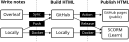
\includegraphics{img/process.svg}
    \else
        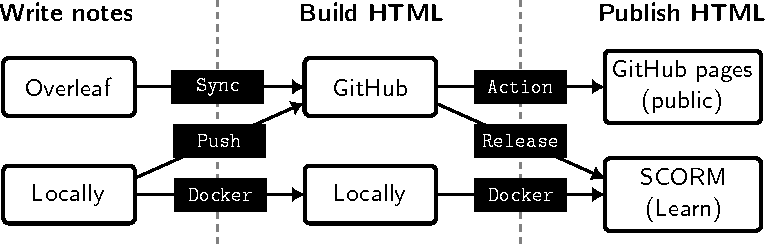
\includegraphics{img/process.pdf}
    \fi
    \caption{Workflow options to build HTML course materials.}
    \alttext{Flowchart showing different workflow options to build HTML course materials.}
    \label{fig:workflow}
\end{figure}

We give detailed guidance for two of these workflows: one with cloud-based conversion and one with local conversion. You can mix-and-match or deviate from these documented workflows if you feel comfortable doing so. If you're not sure where to start, cloud-based is easiest (Section~\ref{sec:github}).


\section{Cloud-based workflow (via GitHub)}
\label{sec:github}

The simplest way to generate HTML course materials makes use of GitHub to perform the conversion in the cloud, which means that you will not need to install anything on your computer. All you need to do is upload your \LaTeX{} source code to a (private) GitHub repository; the conversion to HTML is then done automatically.

Additionally, if you use Overleaf, you can set it up to connect to GitHub. After the initial setup, there will be no need to interact directly with GitHub. Here, we explain this particular workflow\footnote{You should also follow this section if you don't plan to use Overleaf, but still want to use the cloud-based conversion to HTML. The instructions will indicate where to deviate from these steps.}. The main steps are as follows:

\begin{enumerate}[align=left]
    \item[Step 1:] Make a copy of the \href{https://github.com/UoE-School-of-Mathematics/Workflow-Template-Blank}{course notes template from GitHub}.
    \item[Step 2:] Create an Overleaf project, link it to your GitHub repository.
    \item[Step 3:] Write your notes in Overleaf, and sync with GitHub.
    \item[Step 4:] Download the generated HTML version of your notes from GitHub as a SCORM package, and upload it directly to Learn.
    \item[Step 5 (optional):] Easily publish your notes as a public website using GitHub Pages.
\end{enumerate}


\subsection{Step 1: Make a copy of the course notes template on GitHub}
\label{ssec:github}

\subsubsection{Create a GitHub account and join the UoE School of Mathematics organization}

If you already have a GitHub account, then please \href{mailto:lt@maths.ed.ac.uk?subject=Please%20add%20me%20to%20SoM%20GitHub%20organization}{email the Learning Technology Team lt@maths.ed.ac.uk} giving your GitHub username, and ask to be added to the UoE School of Mathematics GitHub organization. 

If you do not have a GitHub account, then please \href{mailto:lt@maths.ed.ac.uk?subject=Please%20add%20me%20to%20SoM%20GitHub%20organization}{email the Learning Technology Team lt@maths.ed.ac.uk} and ask for an invitation to the UoE School of Mathematics GitHub organization. You will receive an email from GitHub with a link to create an account and join the SoM organization. Please note that the email may not render properly in your mail client -- the link may appear as an empty box but this is the invitation link!


\begin{figure}[h]
    \centering
    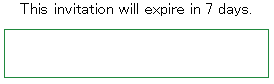
\includegraphics{img/GitHub-invitation.png}
    \caption{GitHub invitation link when it appears empty.}
    \alttext{A blank rectangular box with the text ``This invitation will expire in 7 days'' written above.}
    \label{fig:gh-invitation}
\end{figure}


\subsubsection{Make a new GitHub repository for your notes using the SoM template}

Sign in to your GitHub account, and go to the \href{https://github.com/UoE-School-of-Mathematics/Workflow-Template-Blank}{blank template repository}. Then, click the ``Use this template'' button at the top right of the page. This will create a new repository for you containing the template files.

\begin{figure}[h]
    \centering
    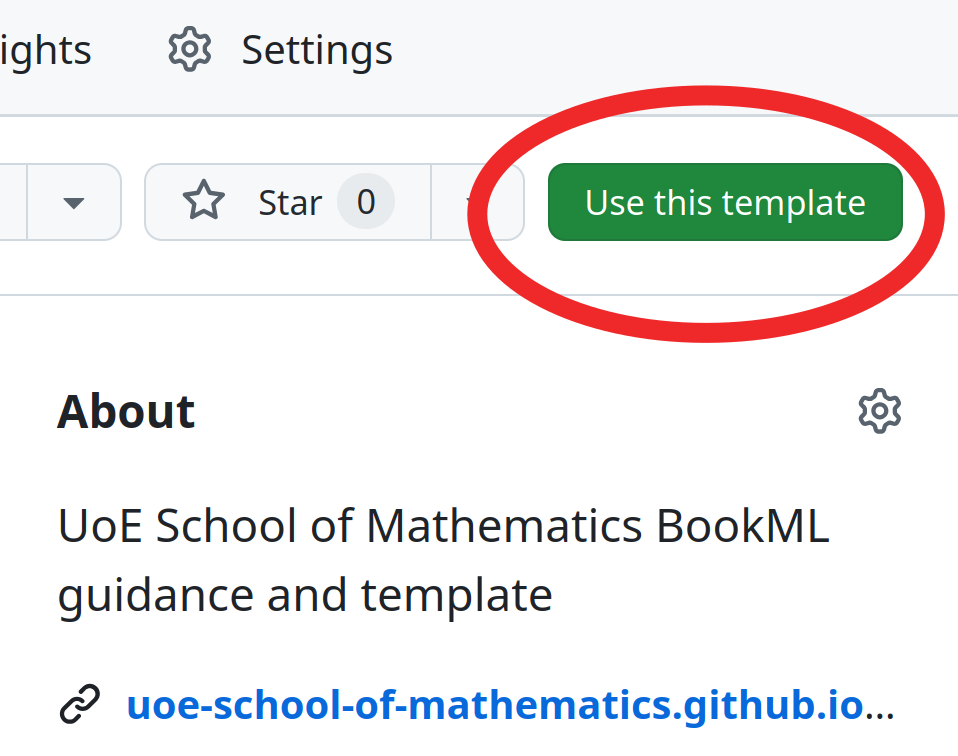
\includegraphics[width=0.5\textwidth]{img/use_template.png}
    \alttext{A screenshot of a webpage showing a green ``Use this template'' button circled in red.}
    \caption{``Use this template'' button is at the top right of the page.}
    \label{fig:use-template}
\end{figure}

The ``Create a new repository'' page has some options:

\begin{itemize}
    \item Keep ``Include all branches'' \textbf{unticked}.
    \item Change ``Owner'' to \textbf{``UoE-School-of-Mathematics''}. This will ensure that your notes are stored in a private repository on GitHub in the UoE School of Mathematics organization\footnote{If you prefer the repository to be owned by your own GitHub account instead, one important difference is that the GitHub Actions minutes needed to perform the HTML conversion in the cloud will be taken from your own GitHub account's quota. The SoM organization has a larger allowance; this is why we encourage you to use it.}.
    \item Choose an appropriate repository name; we recommend that you choose your \textbf{course abbreviation} (e.g. FAC, IMU, IDS, FPM\ldots), or include it in the name.
    \item Make sure ``Visibility'' is \textbf{``Private''}.
\end{itemize}

Finally, click ``Create repository'' and wait at least 3~minutes before moving on. GitHub needs some time to initialise the project.

\subsubsection{Not using Overleaf?}

At this stage, you will have your own copy of the SoM template, as your own repository on GitHub. Steps 2 and 3 below use Overleaf, which makes things easier if you're not familiar with GitHub. However, it's also possible to not use Overleaf at all if you prefer to work locally:

\begin{itemize}
    \item If you are comfortable working with git, you can clone your new repository, and push your changes to GitHub to update the HTML version.
    \item If not, you can also download the files from GitHub (\href{https://docs.github.com/en/get-started/start-your-journey/downloading-files-from-github#downloading-a-repositorys-files}{following these instructions}), extract the .zip, write your notes in that folder, and re-upload any .tex files you have changed directly to GitHub (\href{https://docs.github.com/en/get-started/start-your-journey/uploading-a-project-to-github#step-2-upload-files-to-your-projects-repository}{following these instructions}) every time you want to update the HTML version.
\end{itemize}

In any case, if you do this, you can skip directly to section \ref{ssec:download}.


\subsection{Step 2: Create an Overleaf project linked to your GitHub repository}
\label{ssec:overleaf}

\subsubsection{Link your Overleaf account to your GitHub account}

Visit your \href{https://www.overleaf.com/user/settings}{Overleaf account settings}. Under \textbf{Project Synchronisation}, click \textbf{Link} next to \textbf{GitHub Sync}. Follow the prompts to link Overleaf and GitHub.

\subsubsection{Make an Overleaf project from your GitHub repository}

At this stage, you should have a GitHub repository created from the SoM template. In Overleaf, create a new project, ensuring you choose \textbf{Import from GitHub}. Then, choose \textbf{Import to Overleaf} for the repository you created previously.

\begin{figure}[h]
    \centering
    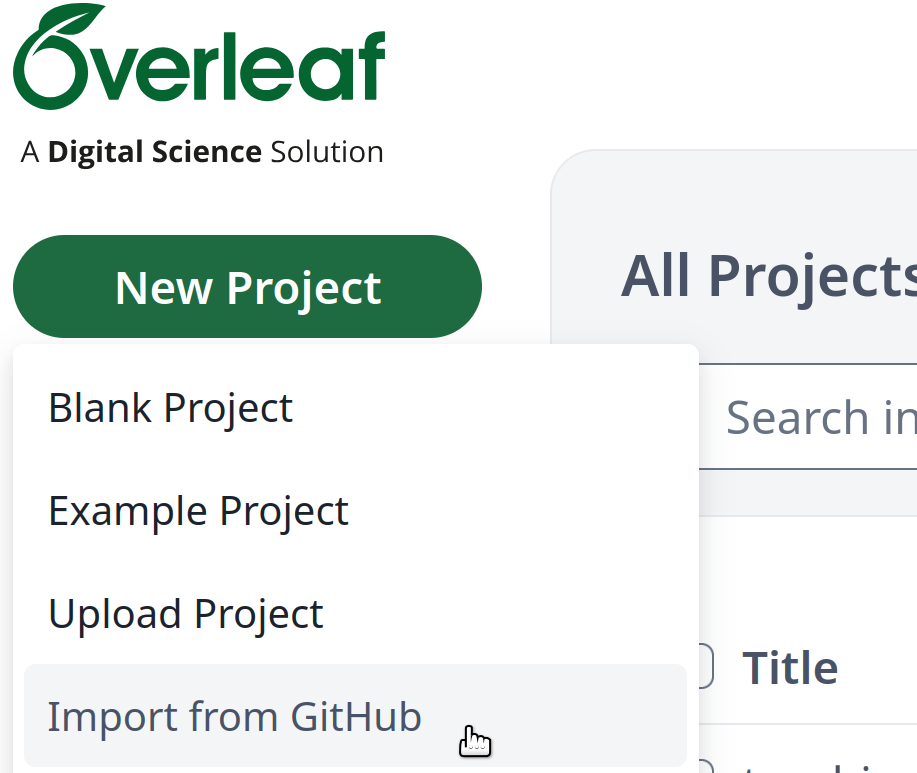
\includegraphics[width=0.5\textwidth]{img/overleaf_new.png}
    \caption{Choose ``Import from GitHub'' when creating the new project.}
    \alttext{A screenshot of the Overleaf ``New project'' options, showing ``Import from GitHub'' selected by the user.}
    \label{fig:gh-overleaf-new}
\end{figure}

Once this is complete, you should have a new Overleaf project containing the template files.


\subsection{Step 3: Write your notes in Overleaf and sync with GitHub}
\label{ssec:sync}

Now you can work on your notes just like with any other Overleaf project.

Whenever you want to publish changes to the HTML version, you need to push the changes to your GitHub repository. To do this, in Overleaf, click \textbf{Menu} (top left) and then choose \textbf{GitHub} under the \textbf{Sync} menu.

\begin{figure}[h]
    \centering
    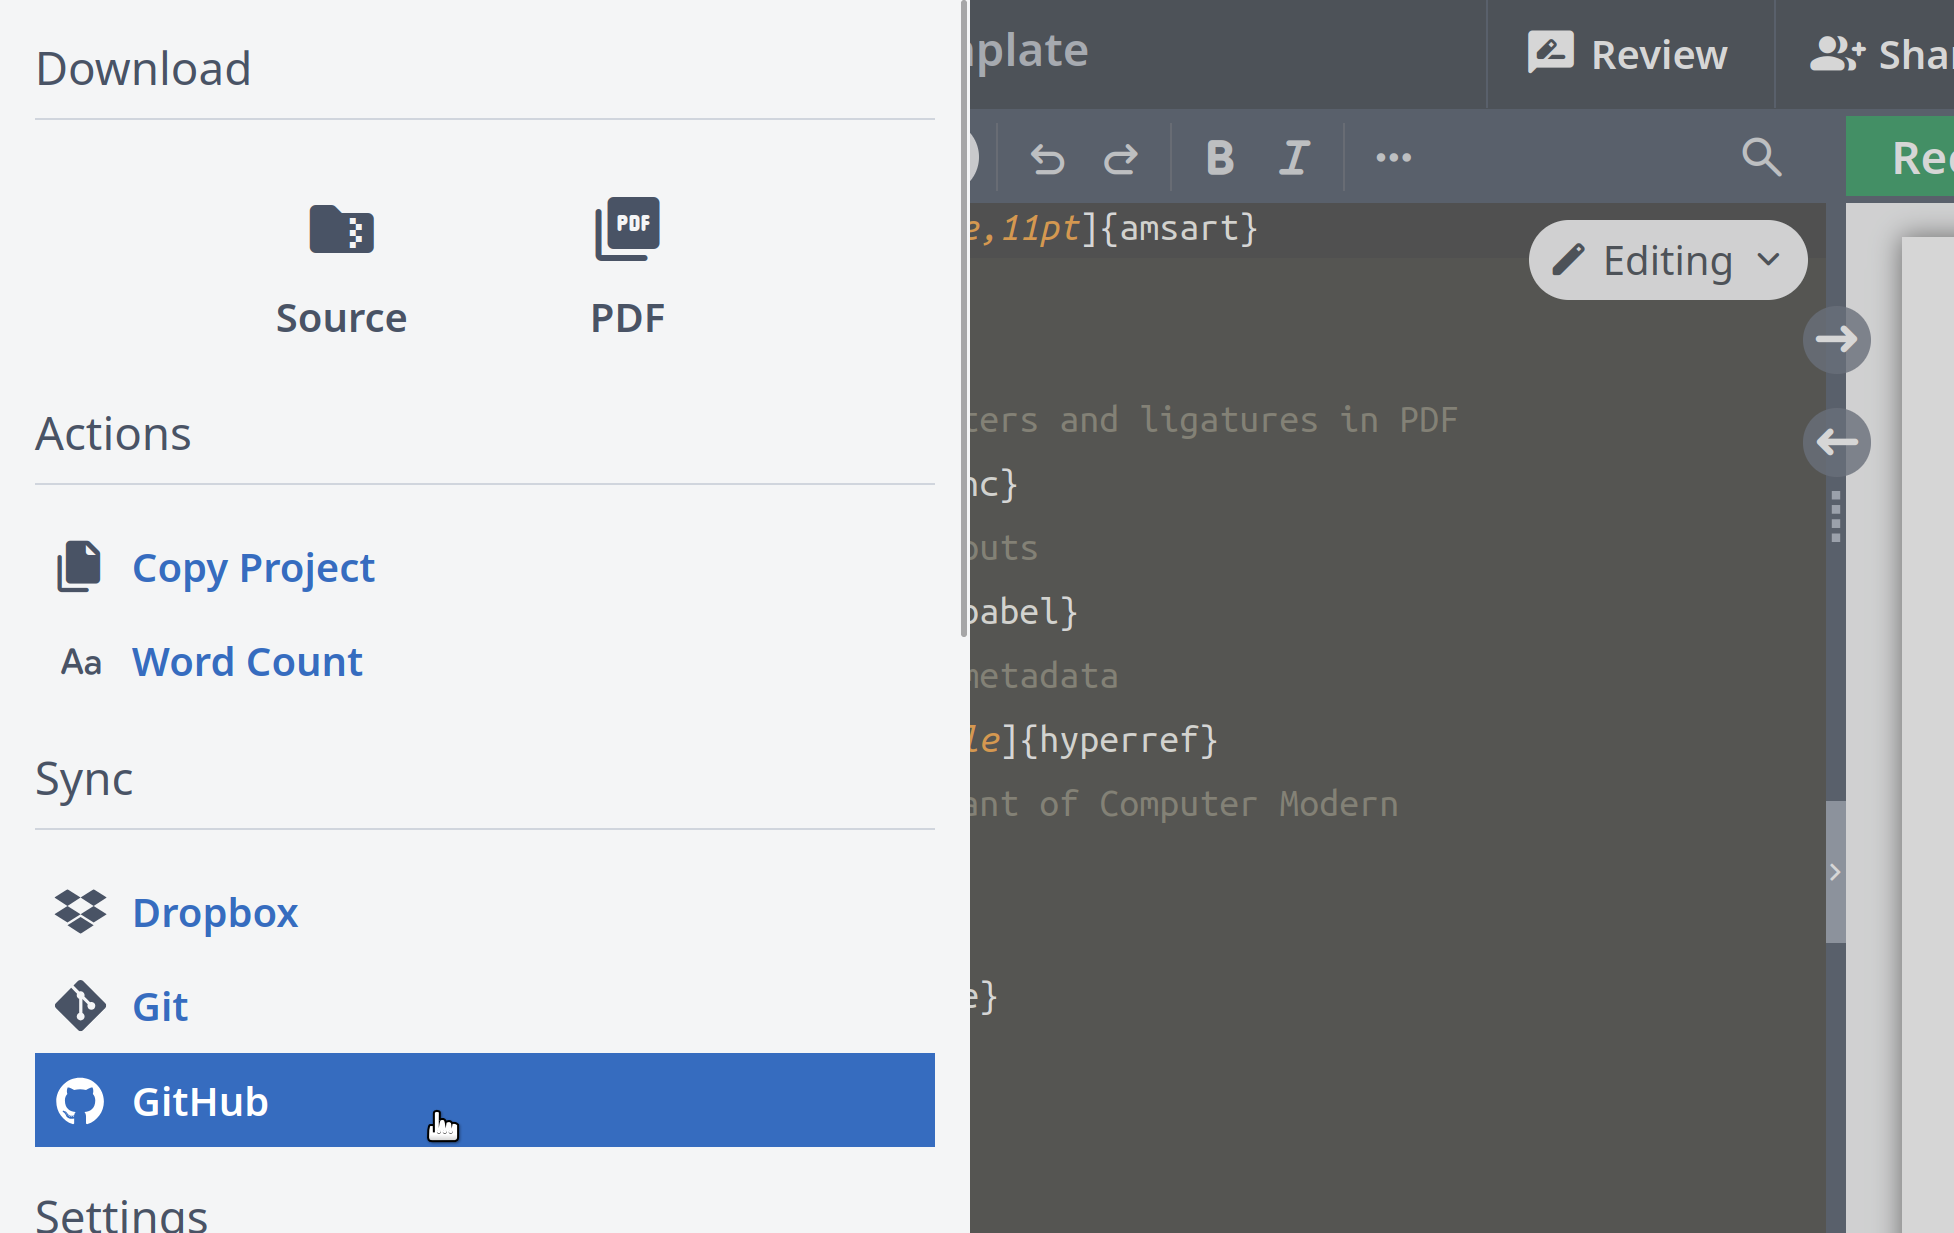
\includegraphics[width=0.6\textwidth]{img/overleaf_sync.png}
    \caption{The ``GitHub'' option in the Overleaf top-left menu.}
    \alttext{A screenshot of the Overleaf menu bar, showing ``GitHub'' selected by the user.}
    \label{fig:gh-overleaf-sync}
\end{figure}

Click \textbf{Push Overleaf changes to GitHub}, enter a description of the changes you have made (optional) and then click \textbf{Sync}.

\subsection{Step 4: Download the generated HTML version of your notes from GitHub as a SCORM package, and upload it to Learn}
\label{ssec:download}

Every time you sync new changes to GitHub, the HTML notes will recompile automatically (this takes a few minutes). Visit your GitHub repository; a green check mark above your files indicates that this has completed. Scroll to ``Releases'' in the right-side menu, and click on the \texttt{SCORM.main.zip} file\footnote{The word \texttt{main} may be replaced by the name of any .tex file with \texttt{documentclass} in it. If you have multiple separate documents in your project, you will get multiple SCORM files to upload on Learn separately.}. This will download a zip file containing the HTML version of your notes.


\subsubsection{Upload the SCORM file}
\label{ssec:scorm}

\begin{itemize}
    \item On your Learn page, create a new content item.
    \item Choose the ``SCORM package'' option.
    \item Upload the file \verb|SCORM.main.zip|.
    \item Once it's uploaded, untick the ``Mark SCORM'' checkbox, and click ``Save''.
\end{itemize}

\begin{figure}[h!]
    \centering
    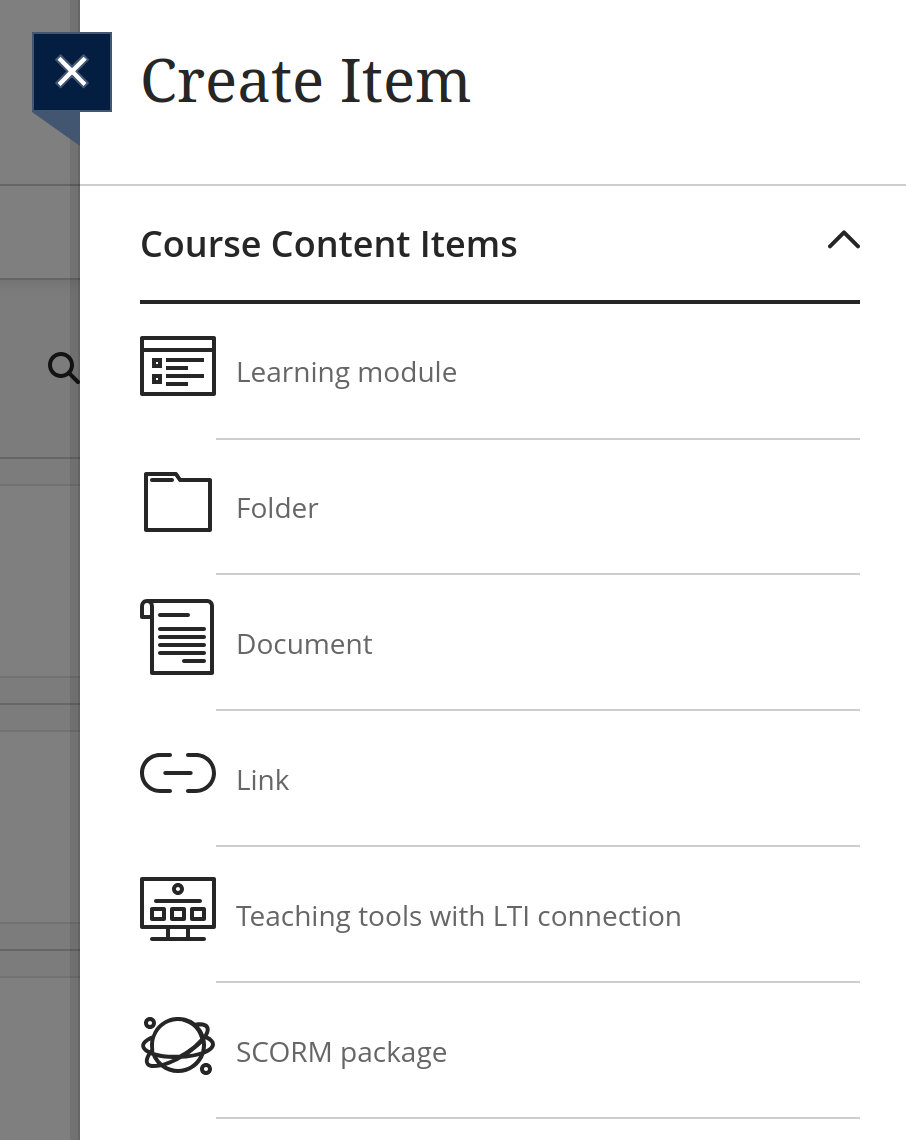
\includegraphics[width=0.5\textwidth]{img/scorm.png}
    \caption{The ``SCORM package'' option on Learn Ultra.}
    \alttext{A screenshot of the ``Create content'' menu on Learn Ultra showing different options. The last option is ``SCORM package''.}
    \label{fig:scorm}
\end{figure}


\subsection{Step 5 (optional): Publish your notes as a public website}
\label{ssec:pub}

Additionally, or alternatively, you can publish your notes as a \textbf{public website} using GitHub Pages. The advantage of doing this, is that this is all already automated; so there is no need for you to manually update your published site every time you update your notes (as you need to do when uploading to Learn). Instead, you can simply add a link to your published website on your Learn page, and this will always point to the most up-to-date version of your notes.

Your site is already built automatically by using the GitHub template, but it's not published by default. To set up a publicly-accessible website with your HTML notes, first visit your repository on GitHub. In the top menu, click \textbf{Settings}, then \textbf{Pages} in the left menu.

Under \textbf{Build and deployment}, look for the \textbf{Branch} option. From the \textbf{Select branch} option, choose \texttt{gh-pages} and \textbf{Select folder} \texttt{/docs}.

\begin{figure}[h]
    \centering
    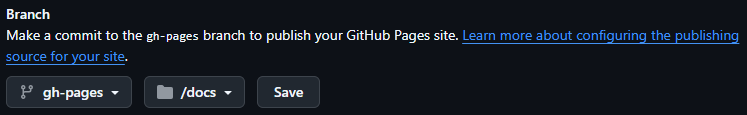
\includegraphics[width=\columnwidth]{img/GitHub-Pages.png}
    \caption{Select the \texttt{gh-pages} branch and the \texttt{/docs} folder.}
    \alttext{A screenshot of a section of the ``Settings'' page. The text reads ``Branch: Make a commit to the gh-pages branch to publish your GitHub Pages site.'' Two drop-down menus and a ``Save'' button are below. The first drop-down menu shows the option ``gh-pages'' was picked. The second shows the option ``/docs''.}
    \label{fig:gh-pages}
\end{figure}

Wait 1~minute then refresh the page. You should now see a link to the publicly-available site hosting your HTML notes. This includes the URL that you should use to share your notes with students.

\begin{figure}[h]
    \centering
    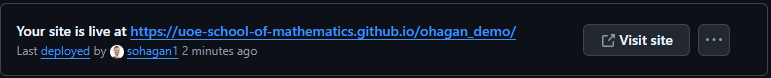
\includegraphics[width=\columnwidth]{img/GitHub-site-link.png}
    \caption{The link to your course site.}
    \alttext{A screenshot of a section of the ``Settings'' page. The text reads: ``Your site is live at https://uoe-school-of-mathematics.github.io/ohagan_demo/'', then ``Last deployed by sohagan1 last month''. There is a ``Visit site'' button on the right.}
    \label{fig:gh-site-link}
\end{figure}

Behind the scenes, GitHub will now automatically rebuild your HTML notes and update the public website every time you synchronise changes with GitHub. This was a one-time setup; you don't need to interact directly with GitHub again.

\subsubsection*{Copyright and license}
\label{ssec:pub:license}

As per UK law, as explained in \href{https://library.ed.ac.uk/library-help/copyright/copyright-teaching}{University guidance}, the University ``is the first owner of the rights of any work made in the course of your employment'', and this applies to teaching materials. By default, this is attributed at the bottom of the index page of your published site.

The University also has an \href{https://open.ed.ac.uk/how-to-guides/}{Open Educational Resources policy and guidance}; we encourage you to consider publishing your course materials as an open educational resource (and change the copyright notice accordingly).


\subsection{Video Guidance}
\iflatexml
Below is a recording of a demo session showing the cloud based workflow. 
\bmlRawHTML{<iframe id="kaltura\_player" type="text/javascript"  src="https://cdnapisec.kaltura.com/p/2010292/embedPlaykitJs/uiconf\_id/55171522?iframeembed=true\&entry\_id=1\_zypgaqqb\&config[provider]=\{'widgetId':'1\_92isimo2'\}"  style="width: 608px;height: 402px;border: 0;" allowfullscreen="" webkitallowfullscreen="" mozAllowFullScreen="" allow="autoplay *; fullscreen *; encrypted-media *" sandbox="allow-forms; allow-same-origin; allow-scripts; allow-top-navigation; allow-pointer-lock; allow-popups; allow-modals; allow-orientation-lock; allow-popups-to-escape-sandbox; allow-presentation; allow-top-navigation-by-user-activation" title="Kaltura Player"></iframe>}
\else
A \href{https://media.ed.ac.uk/media/BookML+LaTeX+to+HTML+Demo+%28recording%29/1_zypgaqqb}{recording of a demo session}
showing the cloud based workflow can be found on media hopper.
\fi


\section{Local workflow}

Another way to create and maintain HTML course materials is to convert your notes locally on your machine. To do this, you will need to either install Docker, or directly install BookML and its dependencies. We give detailed instructions for the Docker workflow, as this is generally easier to set up and use.

\subsection{Using Docker}
\label{ssec:docker}

To run BookML, we can use a Docker container --- a lightweight, portable unit that packages an application and all its dependencies, ensuring that it runs consistently across different environments. This removes the need to download software and maintain dependencies on your computer.

Importantly for us: there is a \href{https://github.com/vlmantova/bookml/pkgs/container/bookml}{Docker image available for BookML}, which is ready-to-use and contains everything we need.

To use it, we can use Docker Desktop, which is available for Windows and Mac, or Docker Engine, which is available for Linux. An open-source alternative (compatible with Docker) is Podman, which is available for Windows, Mac, and Linux. In any case, the key steps are:

\begin{enumerate}
    \item Setup (just once): install Docker or Podman, and download the Docker image.
    \item Convert: run a single command in the folder with your \verb|.tex| files.
\end{enumerate}

Both Docker and Podman allow us to use either the command line or a graphical interface. If you don't know which one to choose, just pick one and try it!

\noindent \textbf{Notes: }
\begin{itemize}
    \item If you have a managed Windows machine, Docker Desktop is available from the software centre. This is a slightly complicated process, 
    see Appendix \ref{app:a} for instructions. It may be simpler to request `Make Me Admin' and install from the internet.
    If you wish to use Podman, you will need to request `Make Me Admin'.
    \href{https://www.ed.ac.uk/information-services/computing/desktop-personal/supported/windows-10/makemeadmin}{Guidance on `Make Me Admin'}.
    \item The Learning Technology team will be able to assist you with installing Docker or Podman --- email \verb|lt@maths.ed.ac.uk| to ask for help.
\end{itemize}

\subsubsection{Setup (first-time only)}
\label{sssec:setup}

\paragraph{Option 1 - to set up Docker:}

\begin{enumerate}
    \item
        \begin{itemize}
            \item \textbf{Windows/MacOS/Linux:} \href{https://docs.docker.com/desktop/install/windows-install/}{Download Docker Desktop from \textbf{this} link} or the Software Centre, and install as instructed by the interface. Launch Docker Desktop. 
There are versions of the download file of Docker Desktop which cause an error. Ensure you are downloading the version that is listed in the documentation.
            \item \textbf{Alternatively for Linux only:} Download and install Docker Engine, following \href{https://docs.docker.com/engine/install/}{the instructions for your distribution}.
        \end{itemize}
    \item Launch a terminal (use \verb|cmd.exe| on Windows), and run the command:\\
        \verb|docker pull ghcr.io/vlmantova/bookml:latest|\\
        This will download the Docker image to your machine.
\end{enumerate}

\paragraph{Option 2 - to \href{https://podman.io/docs/installation}{set up Podman}:}

Note that this requires ``Make Me Admin'' on Windows managed machines.

\begin{enumerate}
    \item \href{https://podman.io/}{Download Podman Desktop from here} and install as instructed by the interface. 
    \item Podman desktop will open, and you will be asked to setup.
    Click the `Setup' button and follow through the instructions 
    that follow. When prompted, select `Yes', and then `Install'. 
    \item Once fully installed, we can download the image. To do this, open the `Images' tab
        (the 4th option on the left-hand side of the screen) and click \verb|Pull| on the top right of the screen, then enter \verb|ghcr.io/vlmantova/bookml:latest| and click ``Pull image''. 
\end{enumerate}

\subsubsection{Conversion}
\label{sssec:conversion}

Before you start, for better results, add \verb|\usepackage{bookml/bookml}| to the preamble of your \verb|.tex| file(s) (after the \textbackslash\verb| documentclass{...}| command). This is not necessary if you are using the \href{https://github.com/UoE-School-of-Mathematics/Workflow-Template-Blank/releases}{template provided here by the School of Mathematics} (download and extract ``Source code (zip)'').

Note that if you use Overleaf, the \verb|bookml/bookml| package will cause an error, unless you also add the \verb|bookml| folder to your project (found in \verb|release.zip| on the \href{https://github.com/vlmantova/bookml/releases}{BookML repository}).

\paragraph{Option (a) - using the command line:}

\begin{enumerate}
    \item Start a terminal in the directory containing your \verb|.tex| file(s). (Use \verb|cmd.exe| in Windows.)
    \item Run the command:\\
        \verb|{software} run -t -v .:/source ghcr.io/vlmantova/bookml:latest|\\
        (replace \verb|{software}| with \verb|docker| or \verb|podman|).
\end{enumerate}

\paragraph{Option (b) - using the graphical interface:}

\begin{enumerate}
    \item In Docker/Podman Desktop, click on the `Images' tab, and you will see the image you have just downloaded. Click the `Play' button (Figure~\ref{fig:docker_desktop_run}).
    \item Under ``Volumes'', specify the ``Host path'' to be the path to your folder, and the ``Container path'' to be \verb|/source|. (In Docker Desktop, this is under ``Optional settings'' -- see Figure~\ref{fig:docker_desktop_path}.)
    % \item In `Optional settings', under `Volumes', in the left box called \verb|Host Path|, copy the path to your folder, or click the three dots to navigate to the folder. In the right box labelled `Container Path', type \verb|/source|.
    \item Click `Run' (Docker) or `Start Container' (Podman) to produce the PDF and HTML outputs.
\end{enumerate}

\begin{figure}[h!]
    \centering
    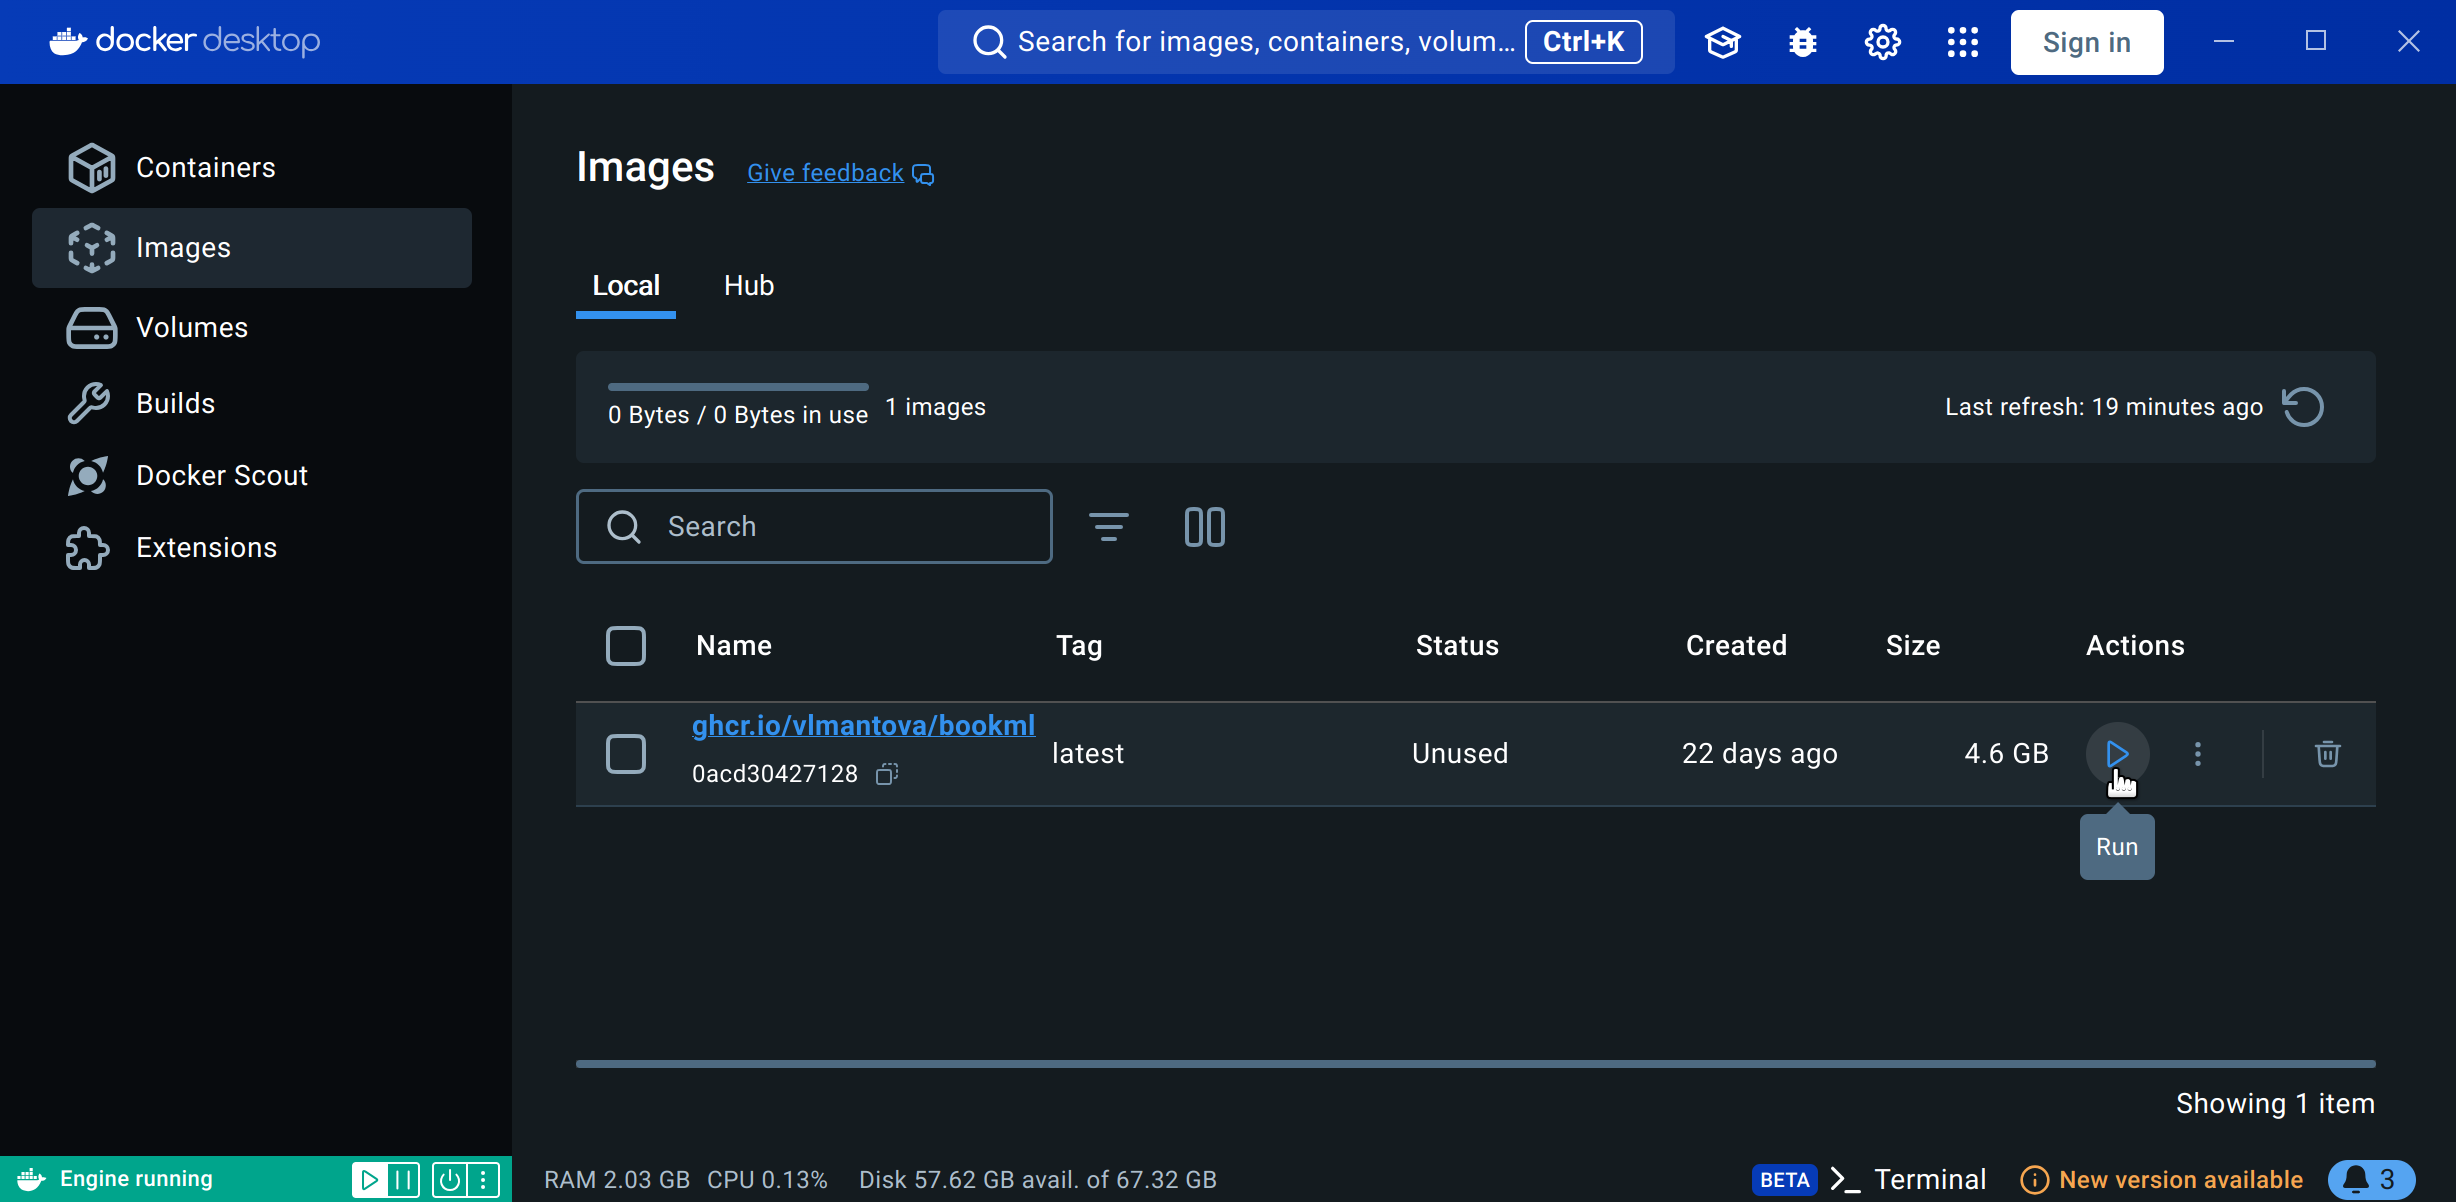
\includegraphics[width=\textwidth]{img/docker_desktop_run.png}
    \caption{Step 1: click the `play' button to run the command.}
    \alttext{A screenshot of Docker Desktop, with the cursor placed on the ``Run'' button.}
    \label{fig:docker_desktop_run}
\end{figure}

\begin{figure}[h!]
    \centering
    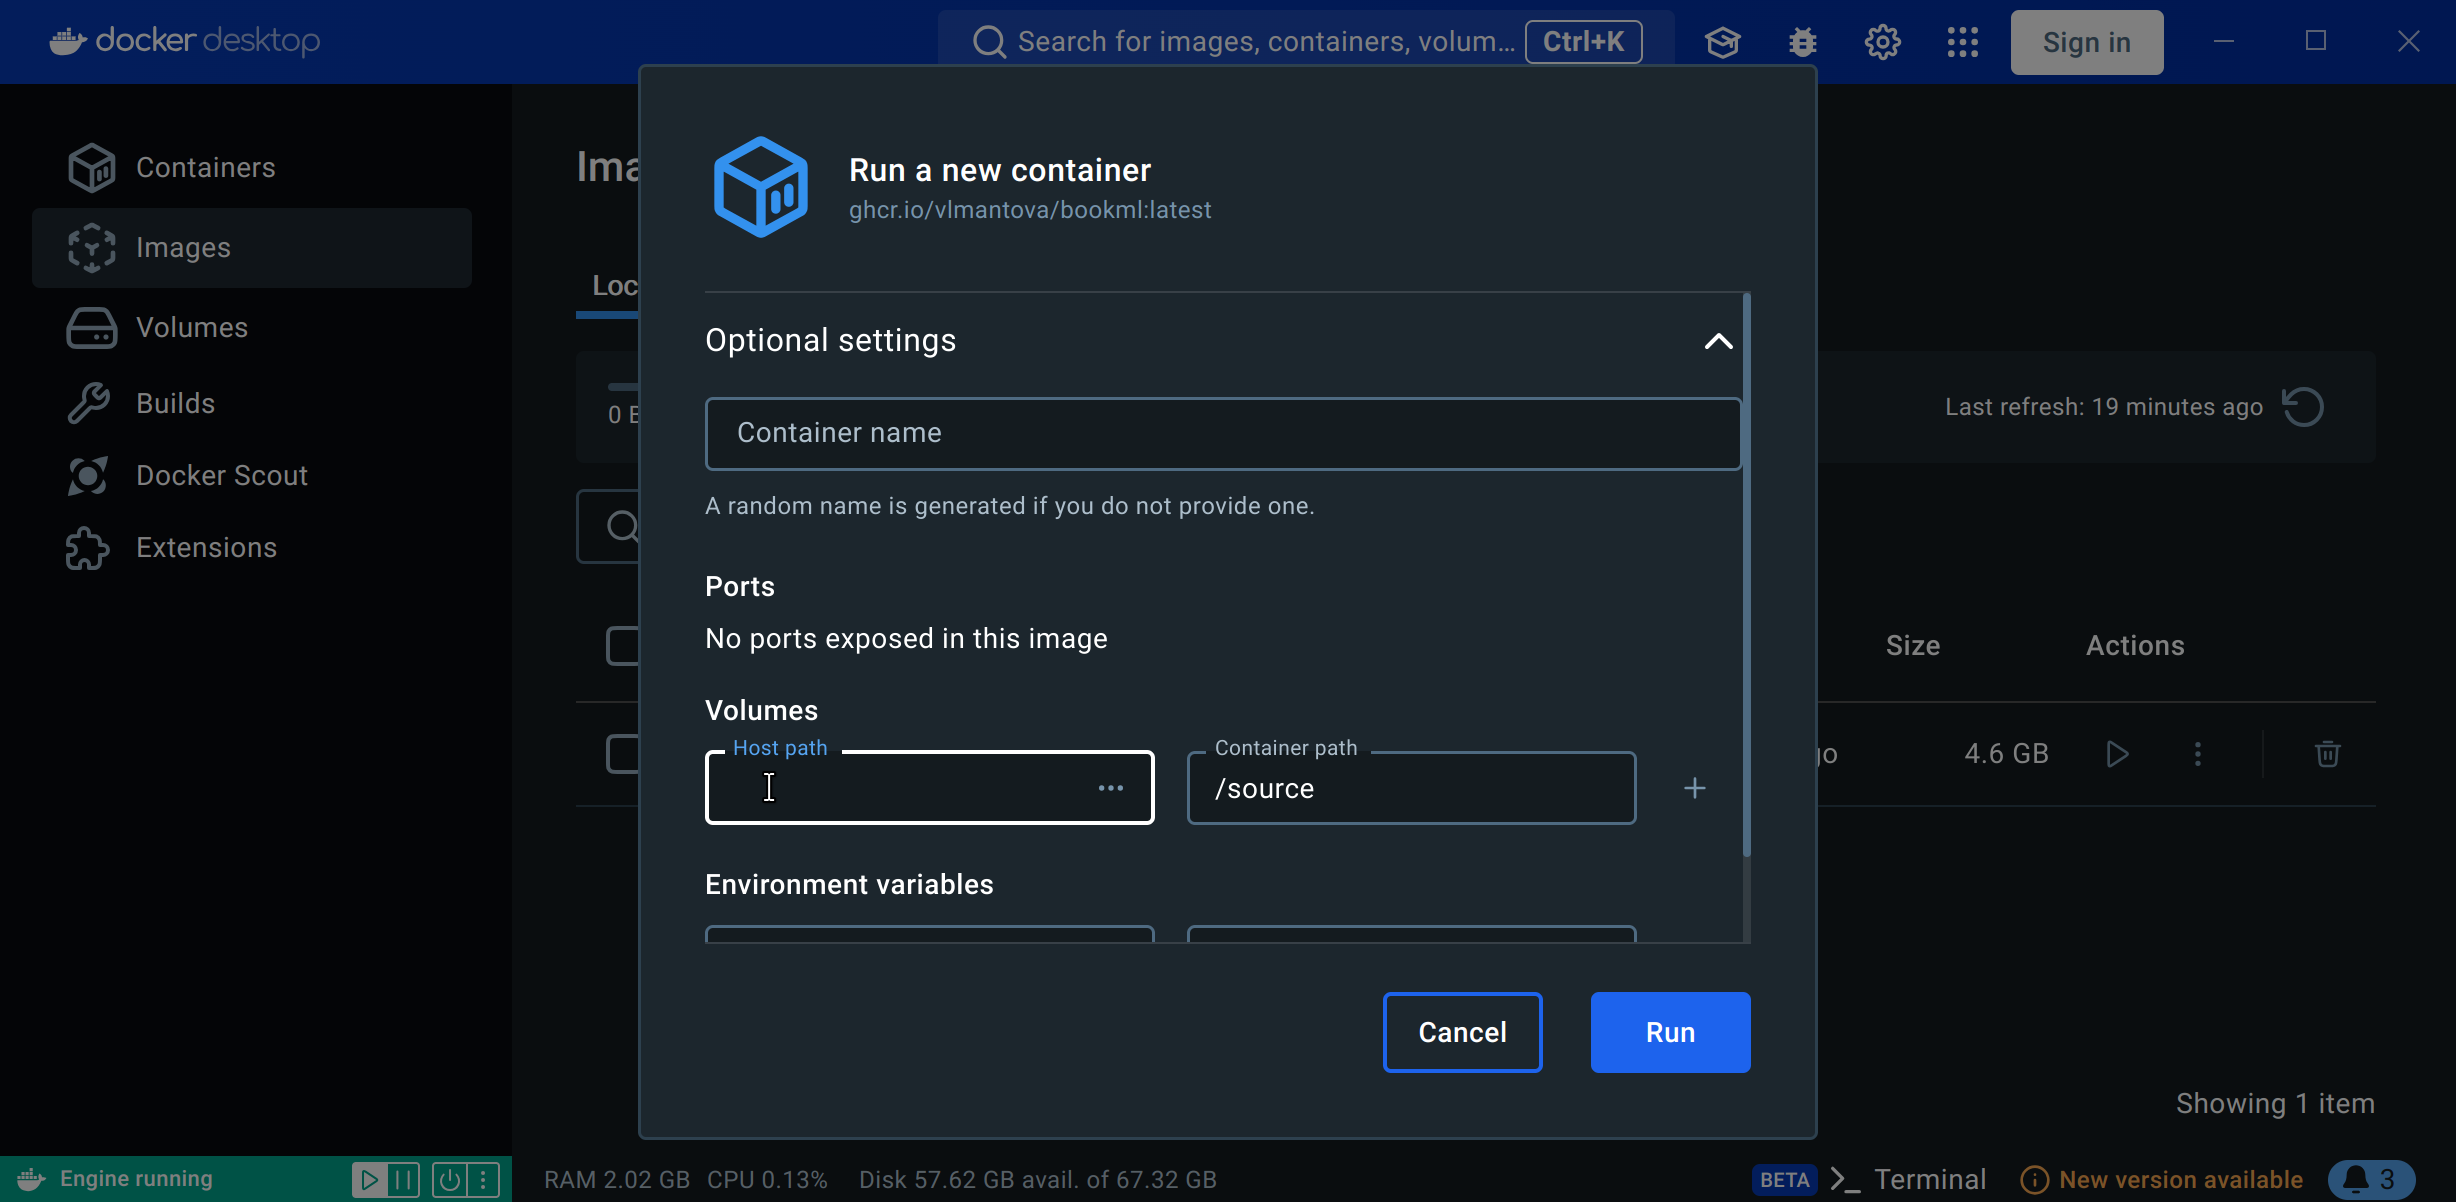
\includegraphics[width=\textwidth]{img/docker_desktop_path.png}
    \caption{Step 2: give Docker the path to your folder.}
    \alttext{A screenshot of Docker Desktop, showing where to input the folder path.}
    \label{fig:docker_desktop_path}
\end{figure}

\subsection{Installing BookML and dependencies manually}
\label{ssec:install}

If you prefer to install the necessary packages and dependencies to your machine instead of using Docker, instructions are given in the \href{https://vlmantova.github.io/bookmlleeds/#S1}{BookML documentation} for the installation and the conversion to HTML.


\subsection{Sharing with students}
\label{ssec:local:share}

Running BookML will produce PDF files (with \verb|pdflatex|), as well as \verb|.zip| files containing the HTML versions of your \verb|.tex| files, which can be uploaded directly to Learn. The output (both PDF and HTML) will be found in the same folder as your \verb|.tex| files.
Upload \verb|SCORM.yourfile.zip| directly to Learn as described in \ref{ssec:scorm}.

The \verb|yourfile.zip| (without the \verb|SCORM|) files contain a standalone HTML site, which you may also wish to publish yourself if you are comfortable doing so (e.g. on your SoM user domain). See \ref{ssec:pub:license} for related copyright information. However, only the \verb|SCORM| versions are fully compatible with Learn, so please use these if you plan to upload your materials to Learn.


\subsection{Learning Technology Mailbox}
\label{ssec:lt}

If you would rather, you can also email \verb|lt@maths.ed.ac.uk| with a .zip of the folder containing all the source files for your course materials (everything needed for your .tex files to compile normally). The Learning Technology team will perform the conversion, and email you back with a .zip file containing the HTML version of your course materials; optionally, they can also upload it to your Learn page. If they spot anything which didn't convert well, they will let you know.


\section{FAQs}
\label{sec:FAQ}

\noindent\textbf{Q: Error: \texttt{Warning: no .tex files with \textbackslash{}documentclass found in this directory}}
\begin{ans}
    The software cannot reach your files, this may be due to running the software in the wrong place, permissions, or a remote directory. 
    Double check your file path, and try moving the files to a local directory and try again.
\end{ans}

\noindent\textbf{Q: Why aren't my files converting at all, there is not an error, BookML simply states there are no files to convert.} 
\begin{ans}
    This is likely due to the fact that the software cannot reach your files. This can be because your files are in a folder, or that your files have \href{https://stackoverflow.com/questions/1976007/what-characters-are-forbidden-in-windows-and-linux-directory-names}{forbidden file characters} or a space.
\end{ans}

\noindent\textbf{Q: The conversion process is taking a very long time.}
\begin{ans}
    The conversion process can take a while, especially for larger documents --- but if it's 30 minutes or more, then please flag this. Note that, if you are using a local installation (not Docker), there are some known issues related to this:
    \begin{itemize}
        \item There is a \href{https://github.com/brucemiller/LaTeXML/issues/2268}{known issue} with the package \verb|expl3| when used with TeXlive 2022 and older which can cause the conversion to take longer.
        \item There is a known issue with the ``postprocessing XSLT'' stage taking several minutes (instead of seconds) on Ubuntu 22.04.
    \end{itemize}
\end{ans}
 
\noindent\textbf{Q: Will my .tex files be converted if I comment out} \verb|\|\verb|documentclass|? 
\begin{ans}
    Yes, and it may cause errors. For files which you don't want to be converted standalone (e.g. files which are \verb|\input|ted into another file), delete the \verb|\|\verb|documentclass| command entirely or move them into a folder.
\end{ans}


\section{Other accessibility information}
\label{sec:otheraccessibility}

This is not the whole picture. There are other things to consider when creating accessible documents that is not handled by materials being in HTML. Additionally, there are other alternatives to a \LaTeX to HTML conversion.

\subsection{Other considerations}
\label{ssec:otheraccessibility}

\begin{itemize}
    \item \textbf{Images:} Ensure that all images have \textit{quality} alternative text. This is not done automatically by BookML, so you will need to add this manually. Information on how to add alt text is in the demo portion of this document (see Section~\ref{demo:fig}), with information about images.
    \item \textbf{Links:} Ensure that all link text is accessible.
    \item \textbf{Use of colour:} Colour should not be used exclusively to communicate information. This is often missed in graphs and charts. For example, portions of a pie chart should be directly labelled, or the legend should be additionally texture-based.
\end{itemize}

\subsection{Alternatives to BookML}
\label{ssec:alternatives}

If you are not strongly attached to using \LaTeX, then instead of using BookML, you can create course materials in accessible formats using \href{https://www.markdownguide.org/basic-syntax/}{the Markdown language}. Software such as \href{https://bookdown.org/}{Bookdown} or \href{https://quarto.org/}{Quarto} offer Markdown support and extended features, and allow you to produce materials in a range of formats (including PDF, HTML, computational notebooks\ldots) directly from Markdown source.

% With these formats you may wish to upload the produced HTML files to Learn. See instructions in Section \ref{appb:zip} for how to upload a zip file to Learn.

% \appendix
% \section{Docker from software centre}
% \label{app:a}
% This method is more complicated than the Docker Desktop download from the internet, but avoids need of admin privileges.
% \begin{enumerate}
    % \item Open the Software Centre and search for Docker Desktop.
    % \item Click on the Docker Desktop icon and click `Install'.
    % \item This download may give the message it has failed, click retry.
    % \item Repeat this a few times, between each download type `docker' into a terminal window and press enter.
     % If docker is installed, the terminal will return a long message about docker commands. If it is not, it will not recognise the command.
    % \item Eventually, the download will prompt a restart. Allow this.
    % \item At this point, leave the machine for an extended time, potentially overnight. 
    % \item After this time, open a terminal window and type `docker' and press enter. 
    % \item Install once again, and the download should be successful. Check using the terminal.
% \end{enumerate}

\chapter{Usage and examples for the template}
\label{demo}

The School of Mathematics provides a default template, which is designed for writing new course materials -- it aims to improve accessibility and convert nicely to HTML. It should also be relatively easy to convert existing materials to this template. The template provides a preamble in \texttt{preamble/SoM.tex}. You can add your own preamble in \texttt{preamble/custom.tex}.

The examples shown in this section are intended to demonstrate the use of the packages and environments included by default in the template, and to give an overview of how different elements are rendered in both the PDF and the HTML versions of a document. Workarounds and \LaTeX\ snippets are also given for certain packages or commands which are not compatible with BookML; these may also be useful to those not using the template.

For more information, see the \href{https://vlmantova.github.io/bookml/#S3.SS1}{BooML Documentation}. This also includes interesting ways of using the HTML functionality.

\section{File structure}
\label{demo:struct}


All content should go either in \texttt{main.tex} (single file), or in separate \texttt{.tex} files located in the same folder as \texttt{main.tex}. If using separate sub-files, they should be included into \texttt{main.tex} using \verb|\input{}|, as is done in this document. Sub-files should \textbf{not} have \verb|\begin{document}| or \verb|\end{document}| commands.

The \texttt{main.tex} template uses the \texttt{book} document class; therefore, the levels of sectioning available are \verb|\part|, \verb|\chapter|, \verb|\section|, \ldots. If you prefer to use \texttt{article} as the document class, then you should use the code in \texttt{main-article.tex~} instead.

You can use \texttt{preamble/custom.tex} to complement the template preamble with any additional packages, macros, custom environments, and so on.


\section{Including or excluding content from either version}
\label{demo:ifpdf}

The \texttt{bookml} \LaTeX{} package includes the command \verb|\iflatexml| to include or exclude particular code from either the PDF or the HTML version of your notes.

\begin{itemize}
    \item Use \verb|\iflatexml| to delimit anything (content, packages, macros, \ldots) that should only be used in the HTML version.
    \item Use \verb|\iflatexml\else| to delimit anything (content, packages, macros, \ldots) that should only be used in the PDF notes.
\end{itemize}

You can check the following example in the source file for this document:

\iflatexml
  \textbf{This will only show up in the HTML version.}
\fi

\iflatexml
\else
  \textbf{This will only show up in the PDF version.}
\fi

\begin{snippet}
\iflatexml
  \textbf{This will only show up in the HTML version.}
\fi

\iflatexml
\else
  \textbf{This will only show up in the PDF version.}
\fi
\end{snippet}




\section{Theorem styles}
\label{demo:thm}

\texttt{preamble/SoM.tex} defines a range of theorem-like styles, and sets up sequential numbering indexed on \texttt{chapter}. Here is an example of a \texttt{theorem} and a \texttt{proof} environment.
Theorem~\ref{th:iterError} and its proof will be in the exam:

\begin{theorem}
  \label{th:iterError}
  Let $\vect{e}_k= \mat{R}^k\vect{e}_0$, for $k\in \mathbb{N}$ and some $\mat{R}\in \R^{n\times n}$. If $\norm{\mat{R}}_p < 1$, then \mbox{$\norm{\vect{e}_k}_p \to 0$} as $k \to \infty$. Change
\end{theorem}

\begin{proof}
  We have
  \begin{align*}
    \norm{\vect{e}_k}_p &= \norm{\mat{R}^k \vect{e}_0}_p \\
    &\leqslant \norm{\mat{R}^k}_p \norm{\vect{e}_0}_p \\
    &\leqslant \norm{\mat{R}}_p^k \norm{\vect{e}_0}_p 
  \end{align*}
  \bmlPlusClass{nolines}
  and so $\norm{\vect{e}_k}_p \to 0$ as $k \to \infty$ if $\norm{\mat{R}}_p < 1$. \qedhere
\end{proof}

Note that the \texttt{align} environment is used in the proof, and also works as expected in the HTML version.

There is also a numbered ``Example'' environment, which has a left-side bar to differentiate it from the rest of the notes. To remove the numbering, see \texttt{SoM.tex}.

\begin{example}
    Let
    \[
        \mat{A} =
        \begin{bmatrix}
            2	&	1	&	1	\\
            4	&	3	&	3	\\
            8	&	7	&	9	\\
        \end{bmatrix}.
    \]
    We want to put $\mat{A}$ into row echelon form. 
    We create zeros below the diagonal in the first column by subtracting multiples of the first row from the other rows:
    \[
        \mat{L}_1 \mat{A} =
        \begin{bmatrix}
            1		&	0	&	0	\\
            -2	&	1	&	0	\\
            -4	&	0	&	1	\\
        \end{bmatrix}
        \cdot
        \begin{bmatrix}
            2	&	1	&	1	\\
            4	&	3	&	3	\\
            8	&	7	&	9	\\
        \end{bmatrix}
        =
        \begin{bmatrix}
            2	&	1	&	1	\\
            0	&	1	&	1	\\
            0	&	3	&	5	\\
        \end{bmatrix}.
    \]
    Repeating this for the second column
    \[
        \mat{L}_2\left(\mat{L}_1 \mat{A}\right) =
        \begin{bmatrix}
            1	&	0		&	0	\\
            0	&	1		&	0	\\
            0	&	-3	&	1	\\
        \end{bmatrix}
        \cdot
        \begin{bmatrix}
            2	&	1	&	1	\\
            0	&	1	&	1	\\
            0	&	3	&	5	\\
        \end{bmatrix}
        =
        \begin{bmatrix}
            2	&	1	&	1	\\
            0	&	1	&	1	\\
            0	&	0	&	2	\\
        \end{bmatrix}
        = \mat{U}.
    \]
    The above procedure factorises $\mat{A}$ as $\mat{A} = \left( \mat{L}_2\mat{L}_1 \right)^{-1}\mat{U}$.
\end{example}

And some extra text after the example to show the return to the regular layout.

If you wish to use a different theorem style, you can do so by editing \texttt{preamble/SoM.tex}. To reflect these changes in the HTML, you can edit the CSS in \texttt{bmluser/SoM.css}. \verb|.ltx_theorem_theorem| is the class for theorems, and \verb|.ltx_theorem_proof| and similar. to edit specifically wish to edit the way it looks in sepia mode or night mode. Add css to \verb|.color-theme-1 .ltx_theorem_theorem| and \verb|.color-theme-1 .ltx_theorem_theorem| respectively.

\subsection{Solutions}

If you wish to hide create a version of the documents with and without solutions, this is generally done using the \texttt{version} package. This is not compatible with BookML. However, we can navigate this with a few options. 

The first choice is to replicate the package using the \texttt{comment} package. Add this code to your preamble. 

\begin{lstlisting}
\iflatexml 
      \usepackage{comment} 
     % \excludecomment{sol} 
      \includecomment{sol} 
\else 
      \usepackage{version} 
      % \excludeversion{sol} 
      \includeversion{sol} 
\fi 
\end{lstlisting}

Alternatively, if you wish to allow students to view solutions but have them hidden, you can use HTML to create a dropdown that students can access with the solution under. Uncomment the following code in \texttt{SoM.tex}.

\begin{lstlisting}
\iflatexml  
    \renewenvironment{solution} 
    {\<details style="text-align: left; width: 100\%" open="">  
    \<summary>  \textbf{Solution}  \</summary>  \\} 
    {\</details> } 
\else 
    \usepackage{version}  
    % \excludeversion{solution}  
    \includeversion{solution}  
\fi 
\end{lstlisting}

This would look like:

\iflatexml  
\<details style="text-align: left; width: 100\%" open="">  \<summary>  \textbf{Solution}  \</summary>  This is how we solve a quadratic.  
    \</details> 
\else 
    \begin{solution}
        This is how we solve a quadratic. 
    \end{solution} 
\fi 




\section{Figures}
\label{demo:fig}

\subsection{Raster images}
\label{demo:fig:raster}

Figure~\ref{fig:coins} is a PNG image included with \verb|\includegraphics|. The \verb|\img| macro is set in \texttt{preamble/SoM.tex}, which you can change there if your graphics folder has a different name.

% Use the \texttt{\includegraphics[alt={alternative text}]{\img/image.png}} to provide \textbf{informative alternative text} for all your images --- this is an \textbf{important accessibility feature}. \href{https://accessibility.huit.harvard.edu/describe-content-images}{Here is useful advice on writing good alternative text}.
Use the command \verb|\alttext{alternative text}| in a \texttt{figure} environment to provide \textbf{informative alternative text} for all your images --- this is an \textbf{important accessibility feature}. \href{https://accessibility.huit.harvard.edu/describe-content-images}{Here is useful advice on writing good alternative text}.

To avoid images being inverted in night mode in HTML, add \verb|\bmlPlusClass{bml_no_invert}| after the \verb|\includegraphics| command. There should be no linebreaks or spaces between. This can also be used for tikz images.

\begin{figure}[H]
    \centering
    % 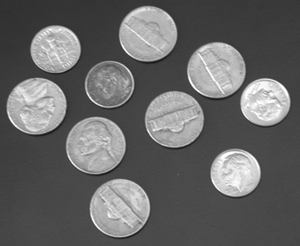
\includegraphics[alt={A greyscale photo of 10 silver coins scattered on a dark grey background.}]{\img/coins.png}\bmlPlusClass{bml_no_invert}
    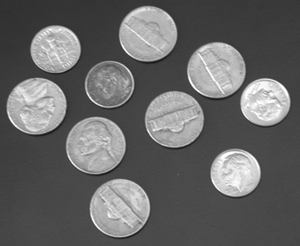
\includegraphics{\img/coins.png}\bmlPlusClass{bml_no_invert}
    \alttext{A greyscale photo of 10 silver coins scattered on a dark grey background.}
    \caption{A PNG image included with \texttt{\textbackslash includegraphics}.}
    \label{fig:coins}
\end{figure}


\subsection{Vector images and diagrams}

\subsubsection{\texttt{tikz} images}
\label{demo:fig:tikz}

Figure~\ref{fig:string} is a \texttt{tikz} diagram included with \verb|\input|.

\begin{figure}[H]
    \centering
    \begin{tikzpicture}[y=0.80pt, x=0.80pt, yscale=-0.7, xscale=0.7, inner sep=0pt, outer sep=0pt]
  \path[draw=black,line join=miter,line cap=round,miter limit=4.00,line
    width=1.200pt] (176.4286,549.5050) .. controls (300.7143,505.2193) and
    (404.2857,517.3622) .. (475.0000,415.2193);
  \path[draw=red,-latex,fill=red,line join=miter,line cap=butt,miter limit=4.00,line
    width=1.200pt] (475.7143,413.0765) -- (507.8571,352.3622);
  \path[draw=red,-latex,fill=red,line join=miter,line cap=butt,miter limit=4.00,line
    width=1.200pt] (174.2857,549.5050) -- (102.1429,571.6479);
  \path[draw=black,dash pattern=on 3.20pt off 3.20pt,line join=miter,line
    cap=butt,miter limit=4.00,line width=0.800pt] (173.5714,548.7908) --
    (97.1429,548.7908);
  \path[draw=black,dash pattern=on 3.20pt off 3.20pt,line join=miter,line
    cap=butt,miter limit=4.00,line width=0.800pt] (476.4286,413.0765) --
    (512.1429,413.0765);
  \path[draw=black,line join=miter,line cap=butt,line width=0.800pt]
    (491.4286,384.5050) .. controls (491.4286,384.5050) and (510.7143,389.5050) ..
    (507.1429,412.3622);
  \path[draw=black,line join=miter,line cap=butt,line width=0.800pt]
    (124.2857,548.0765) .. controls (124.2857,548.0765) and (119.2857,555.9336) ..
    (127.1429,562.3622);
  \path[draw=black,-latex,line join=miter,line cap=butt,miter limit=4.00,line
    width=0.800pt] (88.5714,613.0765) -- (567.1429,613.0765);
  \path[draw=black,dash pattern=on 0.80pt off 1.60pt,line join=miter,line
    cap=butt,miter limit=4.00,line width=0.800pt] (173.5714,549.5050) --
    (173.5714,612.3622);
  \path[draw=black,dash pattern=on 0.80pt off 1.60pt,line join=miter,line
    cap=butt,miter limit=4.00,line width=0.800pt] (475.7143,413.0765) --
    (475.7143,612.3622);
  \path[fill=black] (130.4286,545.0765) node[above right] (text3413)
    {$\theta(x)$};
  \path[fill=black] (490.5714,440.3622) node[above right] (text3417)
    {$\theta(x+dx)$};
  \path[fill=black] (452.8571,636.6479) node[above right] (text3433) {$x+dx$};
  \path[fill=black] (137.8571,582.3622) node[above right] (text3437) {$T$};
  \path[fill=black] (467.7143,386.6479) node[above right] (text3441) {$T$};
  \path[fill=black] (168.7143,636.6479) node[above right] (text3445) {$x$};

\end{tikzpicture}


    \alttext{Diagram of a section of flexible string of length $dx$. Tension is symbolised with a vector T pointing outwards from each end of the string section, at angles theta(x) and theta(x + dx) respectively from the horizontal axis.}
    \caption{Small string element under tension.}
    \label{fig:string}
\end{figure}


\subsection{\texttt{xy} diagrams}
\label{demo:fig:xy}

% The \texttt{tikz-cd} package can also be used to draw commutative diagrams, as an alternative to \texttt{xy}. A \href{https://tikzcd.yichuanshen.de/}{graphical editor is available online}, which generates code. Figure~\ref{fig:cd} shows an example, reproduced from the \href{https://ctan.math.washington.edu/tex-archive/graphics/pgf/contrib/tikz-cd/tikz-cd-doc.pdf}{documentation}.

Figure~\ref{fig:xy} shows an example of a diagram, reproduced from the \href{https://vlmantova.github.io/bookml/#S4.F4}{BookML documentation}.


\begin{figure}
    \begin{bmlimage}
    $$
      \xymatrix{
        U \ar@/_/[ddr]_y \ar@/^/[drr]^x \ar@{.>}[dr]|-{(x,y)} \\
        & X \times_Z Y \ar[d]^q \ar[r]_p & X \ar[d]_f \\
        & Y \ar[r]^g & Z}
    $$
    \end{bmlimage}
    \caption{An example of a \texttt{xymatrix}.}
\end{figure}


\subsubsection{\texttt{pgfplots}}
\label{demo:fig:pgf}

PGF plots are also supported, as shown in Figure~\ref{fig:sqrt}.

\begin{figure}[H]
    \centering
    \begin{tikzpicture}
        \begin{axis}
            \addplot[domain=-3:3, color=blue]{sqrt(x+3)};
        \end{axis}
    \end{tikzpicture}
    \alttext{A plot of sqrt(x+3) between -3 and 3.}
    \caption{Plot created using the \texttt{pgfplots} package.}
    \label{fig:sqrt}
\end{figure}

\subsubsection{SVG}
\label{demo:fig:svg}

Unlike \LaTeX\, HTML can render SVG images directly. If you have SVG images or diagrams as source files, this will produce a clearer image in the HTML version (for example, TikZ images are rendered as SVG). This can be done by using \verb|\iflatexml| to include the SVG image in the HTML version, and the PDF image in the PDF version. This is done below. More information on how this works can be seen in Section~\ref{demo:ifpdf}.

\begin{figure}[H]
    \centering
    \iflatexml
        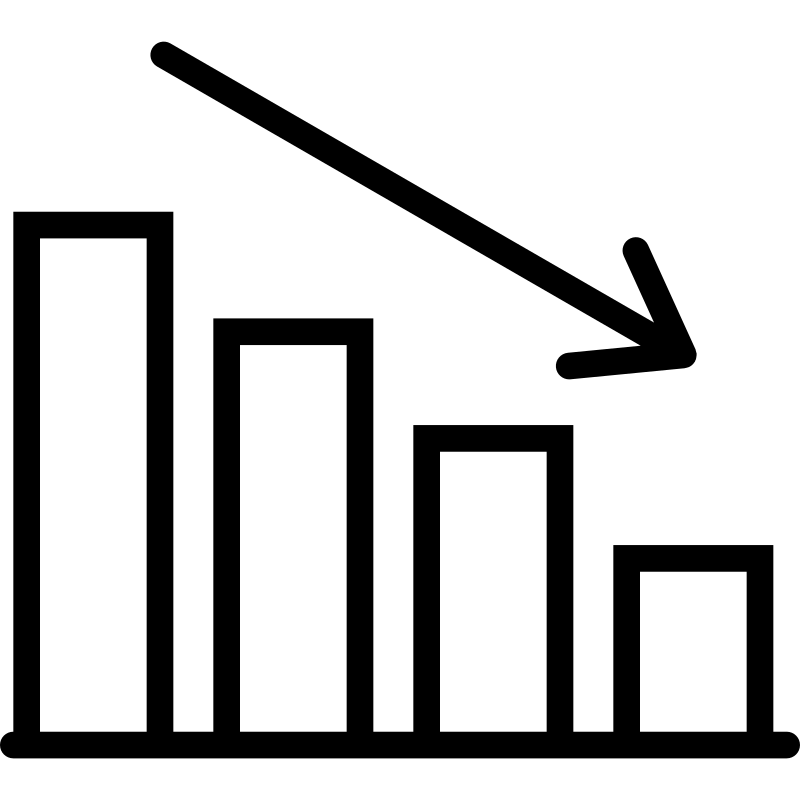
\includegraphics[width=0.25\linewidth]{img/graph.svg}
    \else
        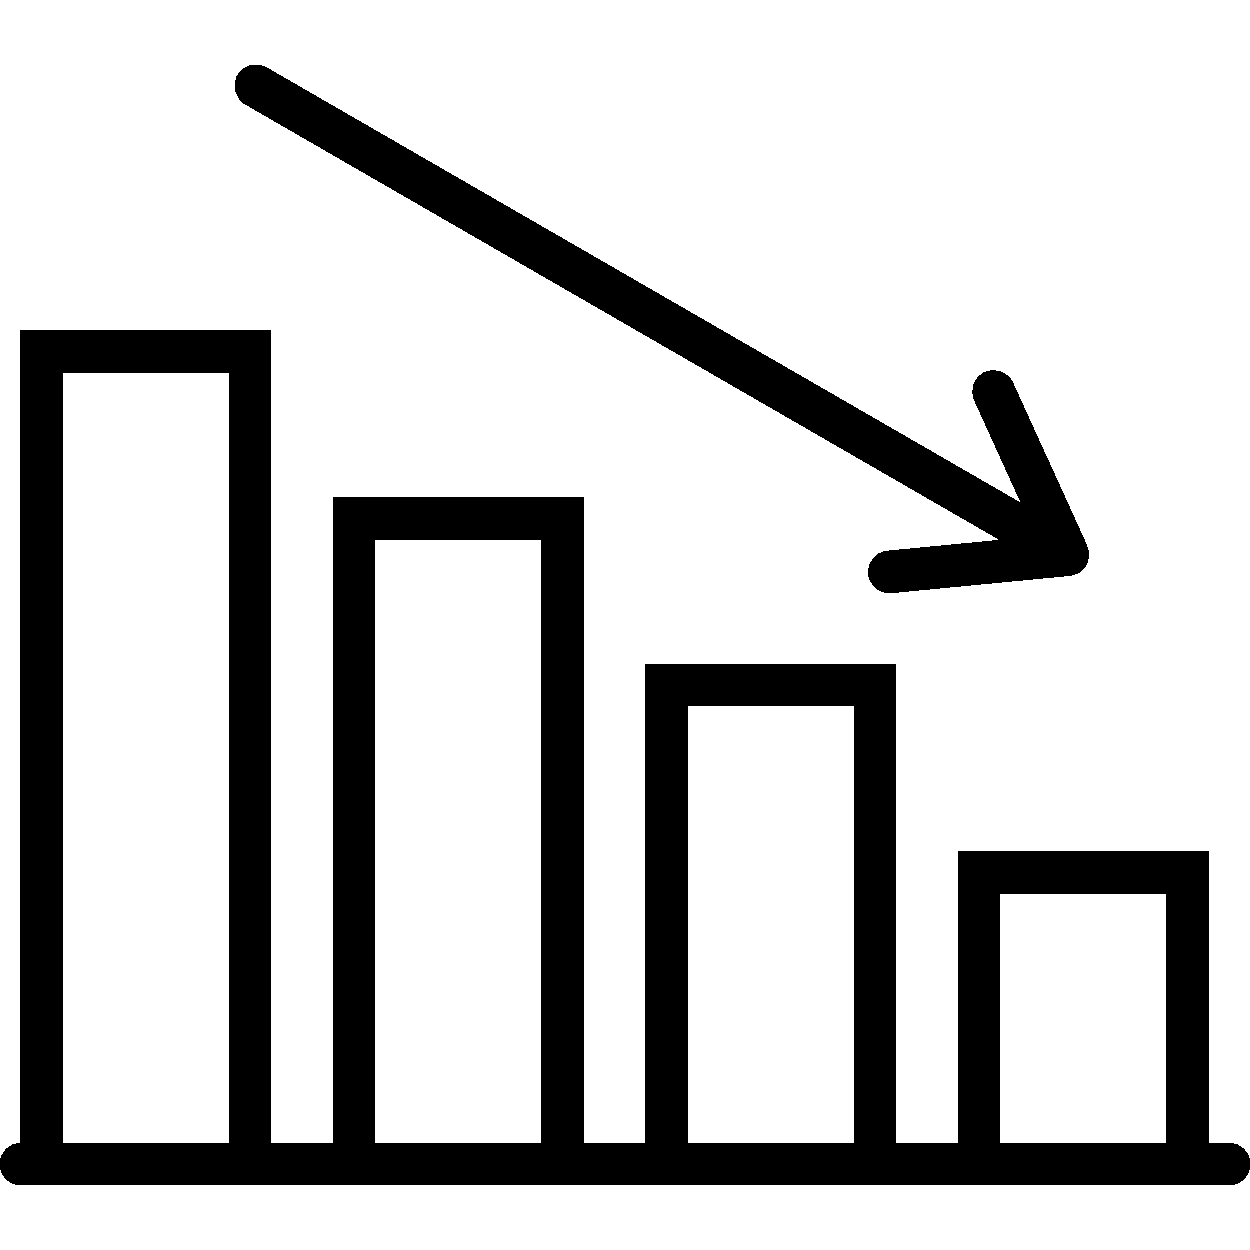
\includegraphics[width=0.25\linewidth]{img/graph.pdf}
    \fi
    \alttext{Generic bar chart with an arrow to indicate downward trend}
    \label{fig:graph}
\end{figure}



\section{Layout}
\label{demo:layout}

\subsection{Subfigures}
\label{demo:fig:subfig}

The \texttt{subfigure} environment from the \texttt{subcaption} package can be used for both the PDF and HTML versions, as seen in Figure~\ref{fig:subs}. Alternatively, the \texttt{minipage} package can be used, as shown in Figure~\ref{fig:minpage}. Unlike \texttt{subcaption}, \texttt{minipage} forces the figures to be side by side, even if they are too wide to fit on the page. This may be useful if you want to force the figures side by side, but you may wish to swap to \texttt{subcaption} for best flow. 

\begin{figure}[H]
    \centering
    \begin{subfigure}{0.35\textwidth}
        \includegraphics[width=\textwidth]{\img/jcmb.jpg}\bmlPlusClass{bml_no_invert}
        \caption{A JPEG image as a subfigure.}
        \alttext{The main entrance of JCMB.}
        \label{fig:jcmb}
    \end{subfigure}
    \hfill
    \begin{subfigure}{0.6\textwidth}
        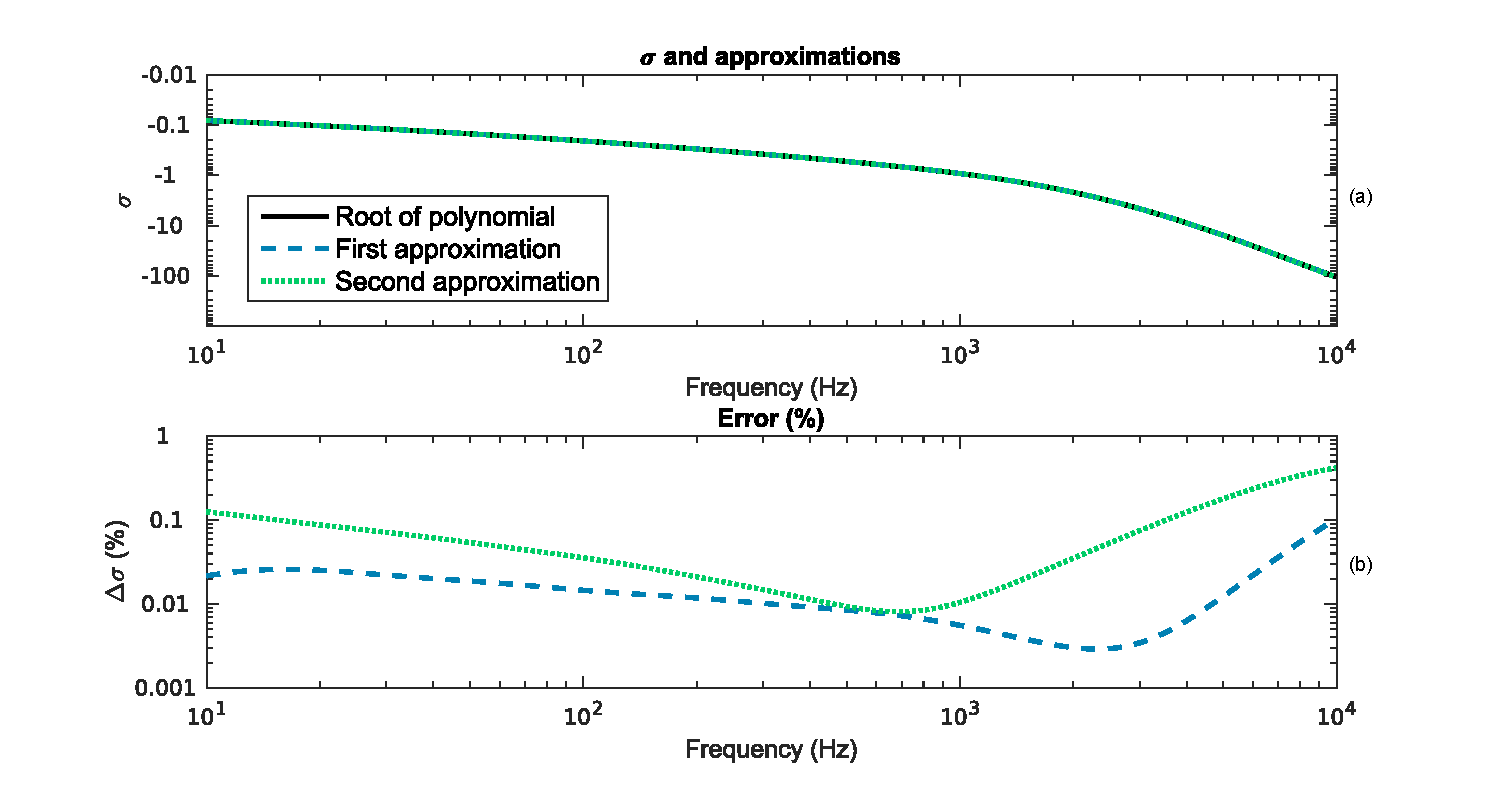
\includegraphics[width=\textwidth]{\img/sigapprox.eps}\bmlPlusClass{bml_no_invert}
        \alttext{Log-log plot showing sigma versus frequency. Three curves overlap almost perfectly: root of polynomial, first approximation, and second approximation.}
        \caption{An EPS file as a subfigure.}
        \label{fig:sig}
    \end{subfigure}
    \caption{Two subfigures,using the \texttt{subcaption} package.}
    \label{fig:subs}
\end{figure}



\begin{figure}[H]
    \centering
    \begin{minipage}{.35\textwidth}
        \centering
        \includegraphics[width=\textwidth]{\img/jcmb.jpg}\bmlPlusClass{bml_no_invert}
        \alttext{The main entrance of JCMB.}
        \caption{A JPEG image as a subfigure.}
        \label{fig:mp-jcmb}
    \end{minipage}%
    \begin{minipage}{0.6\textwidth}
        \centering
        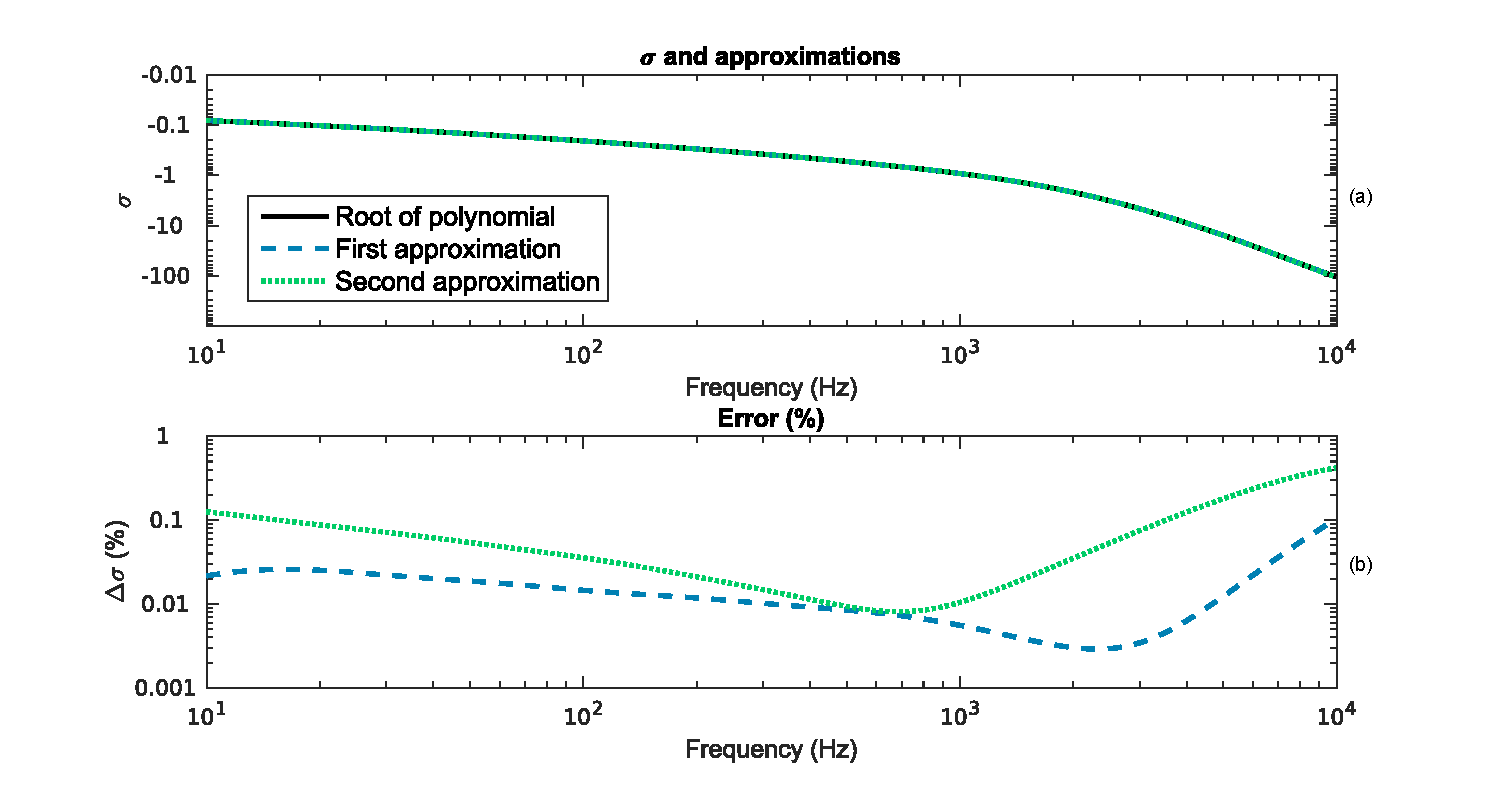
\includegraphics[width=\textwidth]{\img/sigapprox.eps}\bmlPlusClass{bml_no_invert}
        \alttext{Log-log plot showing sigma versus frequency. Three curves overlap almost perfectly: root of polynomial, first approximation, and second approximation.}
        \caption{An EPS file as a subfigure.}
        \label{fig:mp-sig}
    \end{minipage}
    \caption{Two subfigures,using the \texttt{minipage} environment.}
    \label{fig:minpage}
\end{figure}


\subsubsection{Wrapping text around figures}
\label{float:wrap}

\begin{wrapfigure}{r}{0.4\textwidth}
    \centering
    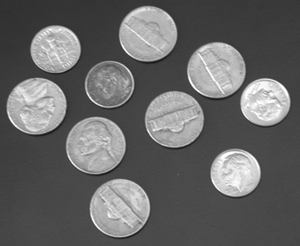
\includegraphics[width=0.35\textwidth]{\img/coins.png}\bmlPlusClass{bml_no_invert}
    \alttext{Photo of 10 silver coins on a dark grey background.}
    \caption{Text wrapped around an image using \texttt{wrapfigure}.}
    \label{fig:wrap}
\end{wrapfigure}

\lipsum[1-2]


\subsection{Tables}
\label{float:tab}

Tables can be typeset using the \texttt{tabular} environment (see Table~\ref{tab:tabular}). Note that the \texttt{tabularx} package is also compatible.

\begin{table}
    \centering
    \begin{tabular}{| l | l | r |} 
      \hline
      cell1 dummy text dummy text dummy text & cell2 & cell3 \\ 
      \hline
      cell1 dummy text dummy text dummy text & cell5 & cell6 \\ 
      \hline
      cell7 & cell8 & cell9 \\ 
      \hline
    \end{tabular}

    \caption{Example table produced with the \texttt{tabular} environment.}
    \label{tab:tabular}
\end{table}


\subsection{Custom floats}
\label{float:custom}

New float types can be created with the \texttt{float} package. For example, Program~\ref{float:prog} is a custom \texttt{program} float (adapted example from the \href{https://en.wikibooks.org/wiki/LaTeX/Floats,_Figures_and_Captions}{LaTeX Wikibooks}). The code is displayed differently but the conversion works.

\begin{program}
  \begin{verbatim}
class HelloWorldApp {
  public static void main(String[] args) {
    //Display the string
    System.out.println("Hello World!");
  }
}
\end{verbatim}
  \caption{The Hello World! program in Java.}
  \label{float:prog}
\end{program}


The package \texttt{multicol} is compatible with BookML, but the in the HTML version, there will not be multiple columns. See bellow, in the PDF version, there are three columns, but in the HTML version, it will be a single column.
\begin{multicols}{3}
     \lipsum[1-2]
\end{multicols}

\section{Other}
\subsection{Multido}
\label{demo:multido}
The \texttt{multido} package is compatible with BookML. It can be used to create loops in your code. For example, the following code will produce a sequence of 8 numbers from 2.00, with a step size of -3.05:

$$
\multido{\n=2.00+-3.05}{8}{\n, }
$$

\subsection{Monospaced output}
\label{demo:code}
The \texttt{listings} package is compatible with BookML. It can be used to create code listings in your document. For example, the following code will produce a listing of a simple Java program:


\begin{lstlisting}[language=Java]
class HelloWorldApp {
  public static void main(String[] args) {
    //Display the string
    System.out.println("Hello World!");
  }
}
\end{lstlisting}
The \texttt{verbatim} environment is also compatible with BookML. It can be used to create verbatim text in your document. For example, the following code will produce a verbatim block of text:

\begin{verbatim}
This is a verbatim block of text.
It will be displayed exactly as it is 
written, with no formatting or special characters such as \LaTeX
\end{verbatim}

\subsection{Referencing from a bibliography}
\label{bib}

The package \texttt{natbib} is compatible with BookML. Note that \texttt{biblatex} is not yet compatible.

This is an example reference~\cite{strikwerda2004}, and another~\citep{parret2016time}. It should not be complex to switch from biblatex to natbib. 




\chapter{Appendicies}
\section{Context: why are we doing this?}\label{sec:context}

The University is legally required to provide learning materials in accessible formats\footnote{\href{https://institute-academic-development.ed.ac.uk/learning-teaching/staff/accessible}{Accessible and Inclusive Learning - University of Edinburgh}}. Although guidance is provided through Information Services\footnote{\href{https://www.ed.ac.uk/information-services/help-consultancy/accessibility/creating-materials}{Creating accessible materials - University of Edinburgh}} for some document formats (e.g., MS Office), workflows deviating from these are not currently supported.

Particularly in subjects which require the extensive use of mathematical notation or other non-standard characters, the \LaTeX\ typesetting language is widely used to generate PDF lecture notes, worksheets, and slides. However, these documents do not currently fulfil accessibility requirements (see Section~\ref{sec:context:PDF}). While there are various approaches to producing accessible documents from \LaTeX\ source files, none of these are widely adopted across the University, or elsewhere. Barriers include technological expertise and means, workload, inconsistent quality of output, and lack of institutional and technical support.

The PTAS project ``A systematic approach to enable production of accessible course materials'' aimed to close this gap by identifying and overcoming such barriers in a systematic manner. Working in collaboration with a diverse community of educators and students, we have developed a set of guidance documents, technical instructions, and \LaTeX\ templates to facilitate the creation of course materials in accessible, flexible output formats.  We have particularly focused on HTML output, which is not only supported by a wide variety of devices, but can also be displayed using user-defined preferences, such as fonts, text sizes, colours, and wrapping for different screen sizes; it is also compatible with many screen readers.


\subsection{Why are PDFs not ``accessible''?}
\label{sec:context:PDF}

In our context, \textbf{accessibility} relates to course content being accessible (as in readable and usable) to everyone, in particular people with disabilities or health conditions. Written content can present accessibility barriers to different people. For example,
\begin{itemize}
    \item those with a visual impairments may use assistive technology (e.g. screen readers) to access course materials;
    \item partially sighted or colourblind people, or those with difficulties related to processing text (for example people with dyslexia or ADHD), may need to customise fonts, font sizes, spacing, and colours to improve accessibility.
\end{itemize}

None of the above is practical to do with PDF files. In particular:
\begin{itemize}
    \item PDF does not allow fonts, sizes or colours to be changed easily;
    \item \LaTeX{}-produced PDF documents are not ``tagged''\footnote{The accessibility checker \textit{Ally}, which is the tool embedded in Learn Ultra, determines the accessibility score of a PDF file largely depending on whether or not it is tagged.} because \LaTeX{} does not (yet) support this feature\footnote{There is ongoing work to improve this at the \LaTeX{} Project, but this is still in early stages; see the paper \href{https://www.latex-project.org/publications/2024-FMi-UFi-TUB-tb139mitt-deims24.pdf}{Enhancing \LaTeX{} to automatically produce
tagged and accessible PDF} for a summary of progress as of March 2024.}. A tagged PDF provides metadata on the document structure, which makes it possible for assistive technologies to navigate between sections --- and therefore makes screen readers usable.
    \item Crucially, screen readers cannot read mathematical expressions inside a PDF file, because the PDF file does not contain any semantic information about the mathematical expressions --- it only contains a graphical rendering of the expressions.
\end{itemize}


\subsection{A solution: HTML with MathML}
\label{sec:context:HTML}

HTML documents are accessible in some ways that PDF documents are not.
\begin{itemize}
    \item The user can easily change font size, font family, and colours\footnote{This can be done with custom style sheets (for instance via browser extensions such as \href{https://add0n.com/stylus.html}{Stylus}), or Javascript (for example, try the toolbar at the top of the HTML version of this document).}. It is also possible to print from HTML to paper while conserving your font settings -- so you can print in large font, for example (which, again, is not straightforward with a PDF).
    \item The document structure and navigation relies on HTML tags, which are accessible by screen readers.
    \item Providing alternative text (or alt-text) for figures is easier. This is different from figure captions --- it describes the key features of a figure under the assumption that the person reading the alt-text cannot see the image.
    \item Mathematical expressions are displayed using MathML\footnote{\href{https://www.w3.org/Math/}{MathML homepage}}, which is compatible with a range of assistive technologies (e.g. screen readers and Braille displays)\footnote{\href{https://www.chhs.colostate.edu/accessibility/best-practices-how-tos/mathml/}{Brief explanation and demonstration of MathML, including a video showing use with a screen reader}.}.
\end{itemize}

MathML renders all mathematical expressions in a document, whether inline ($x = 1$) or in display mode:

\begin{equation}
    \label{eq:mathjax}
    f(x) = \int_{0}^{\infty} \left( \frac{e^{-t^2}}{\sqrt{\pi}} \right) \left( \sum_{n=0}^{\infty} \frac{(-1)^n x^{2n+1}}{(2n+1)!!} \right) \, dt
\end{equation}

You may be familiar with MathJax\footnote{\url{https://www.mathjax.org/}}, used for instance on STACK. MathJax is a Javascript engine used to display MathML in the browser. \href{https://andrewlock.net/rendering-math-in-html-mathml-mathml-core-and-asciimath/}{This is a good primer} on what they both do. In particular, MathJax offers a contextual menu on right-click with further accessibility features, including the possibility to copy the \LaTeX{} source for an expression (try it with the expression above, in the HTML version of this document).

It is possible to generate HTML with MathML \textit{automatically} from \verb|.tex| source files --- so we don't have to worry about doing any of this manually. A key part of the PTAS project was to review different workflows for doing so, in order to provide recommendations and appropriate support for robust, user-friendly production of accessible course materials.


\subsection{Insights from staff interviews}
\label{sec:interviews}

During the Spring semester of 2023--24, we conducted interviews with teaching staff from the Schools of Mathematics, Physics and Astronomy, Engineering, and Philosophy, Psychology, and Language Sciences to better understand their current workflows in producing course materials. We specifically chose staff members who work extensively with \LaTeX{}.

Several common themes emerged from these discussions, which helped inform our approach:

\paragraph{Teaching staff have limited time.} Any proposed adjustments must be integrable into existing workflows with absolutely minimal increase in workload. Solutions should prioritize simplicity, efficiency, and robustness, without the need to extensively consult documentation or complex instructions. Technical support should be provided to resolve problems.

\paragraph{Openness to adjustments in workflow.} While the staff we interviewed expressed willingness to adjust their workflows to enhance accessibility of their materials, this may well be biased by us interviewing staff who put themselves forward to discuss this in the first place. This underscores the importance of making all recommendations user-friendly and low-friction to ensure widespread adoption.

 \paragraph{Challenges of shared \LaTeX\ documents.} Documents in \LaTeX\ authored by multiple contributors or handed down over time often exhibit inefficiencies such as redundant or inefficient use of packages. Additionally, they may contain large blocks of commented-out code from previous versions or authors, which can clutter the document and complicate maintenance. These remnants, while intended for reference or future use, often become outdated and may not serve future iterations of the document effectively. Such practices can hinder readability, increase file size, and make it challenging to navigate and update course materials efficiently.

\paragraph{There are more similarities than differences.} While a multitude of resources are employed in creating course materials, the majority of \LaTeX\ documents typically share similar foundational structures. Variations typically arise from specialized packages tailored to specific subjects, use of different engines to compile PDFs, the number of authors involved, and other contextual factors. This implies that supporting solutions which accommodate different packages, custom macros, and figures/images will enable us to develop a solution applicable to a wide range of \LaTeX\ documents.


\section{Flexibility is the key}
\label{sec:context:flex}

A driving principle we choose to adopt in this project is \textbf{flexibility}, both on the side of the users (usually students) and producers (usually lecturers) of course materials.

\begin{itemize}
    \item Writers of course materials should be able (and appropriately supported) to produce accessible versions with as little change to their preferred workflow as possible. In any automatic conversion process, technical issues and incompatibilities are inevitable --- but technical support, consultation, testing, and iterative refinement will drastically help to reduce this.
    \item Users should be able (and appropriately supported) to customise the display of course materials to a format that is most accessible to them. There are certainly general guidelines we can follow to produce accessible documents --- but prescribing a specific format (e.g. prescribing a specific font family or colour palette) is not as good as giving people options.
\end{itemize}

Importantly: accessibility is about ensuring that \textbf{everyone} can engage fully. For instance, for many students, PDF course materials will always be their preferred option: they are useful for printing, annotating and note-taking on tablets, and can be easier to use offline. We are very much \textbf{not asking lecturers to get rid of their PDF notes} unless they want to --- the idea is to also provide alternative options.

\section{Upload as ZIP}
\label{appb:zip}

You can upload a \verb|.zip| file directly to the Content Collection on your Learn page, as a ``zip package''. PLease note this method will not work if you upload the \verb|.zip| file to your general content collection, rather than on the direct on the specific learn page.

This should only be done if there is no option to upload a SCORM version of the materials.

\begin{enumerate}
    \item On your main Learn page, click the \verb|+| button to add content, then select `Content Collection' at the bottom.
    \item Select `Browse content collection'.
    \item At the top, click `Upload', then `Upload zip package'.
    \item Select `Browse local files' and select the \verb|.zip| file you have just created, or drag and drop the file into the box.
    \item Click `Submit'.
    \item Click on the folder you have just uploaded, check the box next to \verb|index.html| and click `Submit'. 
    \item Click on the \verb|...| on the right to change the name from \verb|index.html| to something more helpful for students (e.g. ``Course notes''), and click `Save'.
\end{enumerate}

\textbf{Important}: with this method, you then need to add permission to the folder for students to view the whole site.

\begin{enumerate}
    \item From the Learn home page, select ``Tools'', then ``Content Collection''.
    \item Click on the folder corresponding to your course.
    \item Hover on the folder containing your HTML course materials, click the arrow to get the contextual menu, and select ``Permissions''.
    \item Click on ``Select Specific Users by Place'', then ``Course''.
    \item Tick the name of your course, then tick ``All course users'' below.
    \item Tick the ``Read'' option, leave the others unticked, and also leave ``Overwrite'' unticked.
    \item Click ``Submit''.
\end{enumerate}




%\part{Second part}

\appendix
% Include appendix "chapters" here.



\backmatter
%    Bibliography styles amsplain or harvard are also acceptable.
\bibliographystyle{amsalpha}
\bibliography{biblio}
%    See note above about multiple indexes.
%\printindex

\end{document}

%-----------------------------------------------------------------------
% End of main-book.tex
%-----------------------------------------------------------------------

